\documentclass{beamer}

\usepackage{graphicx} % Required for inserting images
\usepackage{xeCJK}
\usepackage{amsmath, amssymb, amsthm, amsfonts}
\usepackage{unicode-math}
\usepackage{algorithm}
\usepackage{algpseudocode}
\usepackage{multirow}
\usepackage{siunitx}
\usepackage{animate}
\usepackage{subcaption}

%,algorithm2e,float
\usepackage{hyperref}

\usepackage{biblatex}
\addbibresource{ref.bib}

% Define operator
\DeclareMathOperator*{\argmax}{argmax}
\newcommand{\algorithmicbreak}{\textbf{break}}

%theme settings

%\usetheme{Madrid}
%\usetheme{Ilmenau}
%\usetheme{Berlin}
%\usetheme{Darmstadt}
\usetheme{Frankfurt}
%\usetheme{Ilmenau}
%\usetheme{Singapore}

\usecolortheme{default}
\definecolor{UQmain}{rgb}{0.4,0.8,0.4}
\setbeamercolor*{palette primary}{bg=UQmain, fg=white}
\setbeamercolor*{palette secondary}{bg=white, fg=UQmain}
\setbeamercolor*{palette tertiary}{bg=UQmain, fg=white}
\setbeamercolor*{palette quaternary}{bg=UQmain, fg=white}
\AtBeginEnvironment{thm}{%
    \setbeamercolor{block body}{bg=white, fg=black}
    \setbeamercolor{block title}{bg=UQmain, fg=white}}


\setCJKmainfont{AR PL UKai TW}
% 這兩行一定要加，中文才能自動換行
\XeTeXlinebreaklocale "zh" 
\XeTeXlinebreakskip = 0pt plus 1pt



\title{Probability of Informed No-Tradings: \\
A Copula-Based PIN Model with Zero-Inflated Poisson Distributions}
\author[]{Chu-Lan Kao \inst{1} \and Emily Lin \inst{2} \and Shan-Chi Wu \inst{3}}
\institute[]{\inst{1} Institue of Statistics, National Yang Ming Chiao Tung University, Taiwan \and \inst{2} Department of Fashion Administration and Management, St. John's University, Taiwan \and \inst{3} Institute of Statistical Science, Academia Sinica, Taiwan}



%\advisor{Chu-Lan Michael Kao}
\date{May 27, 2024}%\today

\begin{document}

\begin{frame}
    \maketitle
\end{frame}

\begin{frame}{Outline}
    \tableofcontents
\end{frame}


\section{Introduction}

\begin{frame}{Introduction}
    \begin{itemize}
        \item The probability of informed trading (PIN) models is widely used to determine the information asymmetry in the security market.
    \end{itemize}
    
    \begin{figure}
        \centering
        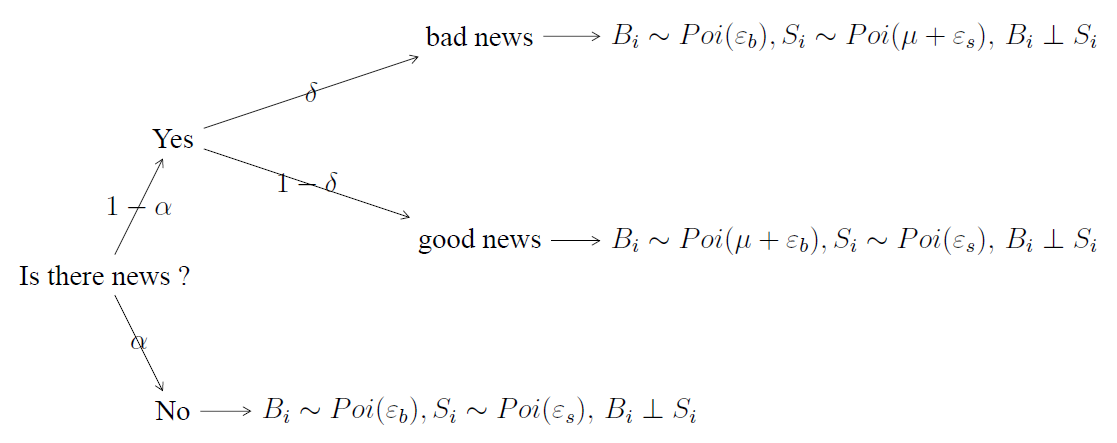
\includegraphics[width=\textwidth]{figures/PIN.png}
        \caption{The structure of the PIN model}
        \label{PIN}
    \end{figure}
\end{frame}

\begin{frame}{Introduction}
    Regard the classical PIN model as a mixture model:
    \begin{equation*}
    \begin{split}
    f(B,S|\theta) &= (1-\alpha) e^{-\varepsilon_b} \frac{\varepsilon_b^B}{B!} e^{-\varepsilon_s} \frac{\varepsilon_s^S}{S!} \\
    &+ \alpha\delta e^{-(\mu+\varepsilon_b)} \frac{(\mu+\varepsilon_b)^B}{B!} e^{-\varepsilon_s} \frac{\varepsilon_s^S}{S!} \\
    &+ \alpha(1-\delta) e^{-\varepsilon_b} \frac{\varepsilon_b^B}{B!} e^{-(\mu+\varepsilon_s)} \frac{(\mu+\varepsilon_s)^S}{S!},
    \end{split}
    \end{equation*}
    where $\theta = (\alpha,\delta,\mu,\varepsilon_b,\varepsilon_s)$.
    \smallskip
    
    For parameter estimation, using the EM algorithm.
    \begin{equation*}
        \hat{\theta}_\text{MLE} = \argmax_\Theta \sum_{i=1}^n L(\theta|B_i,S_i)
    \end{equation*}
\end{frame}


\begin{frame}{Introduction}
    \begin{itemize}
        \item The model assumption is that the correlation between buys and sells is independent $\longrightarrow$ not reasonable in empirical.  
    \end{itemize}
    
    \begin{figure}
        \centering
        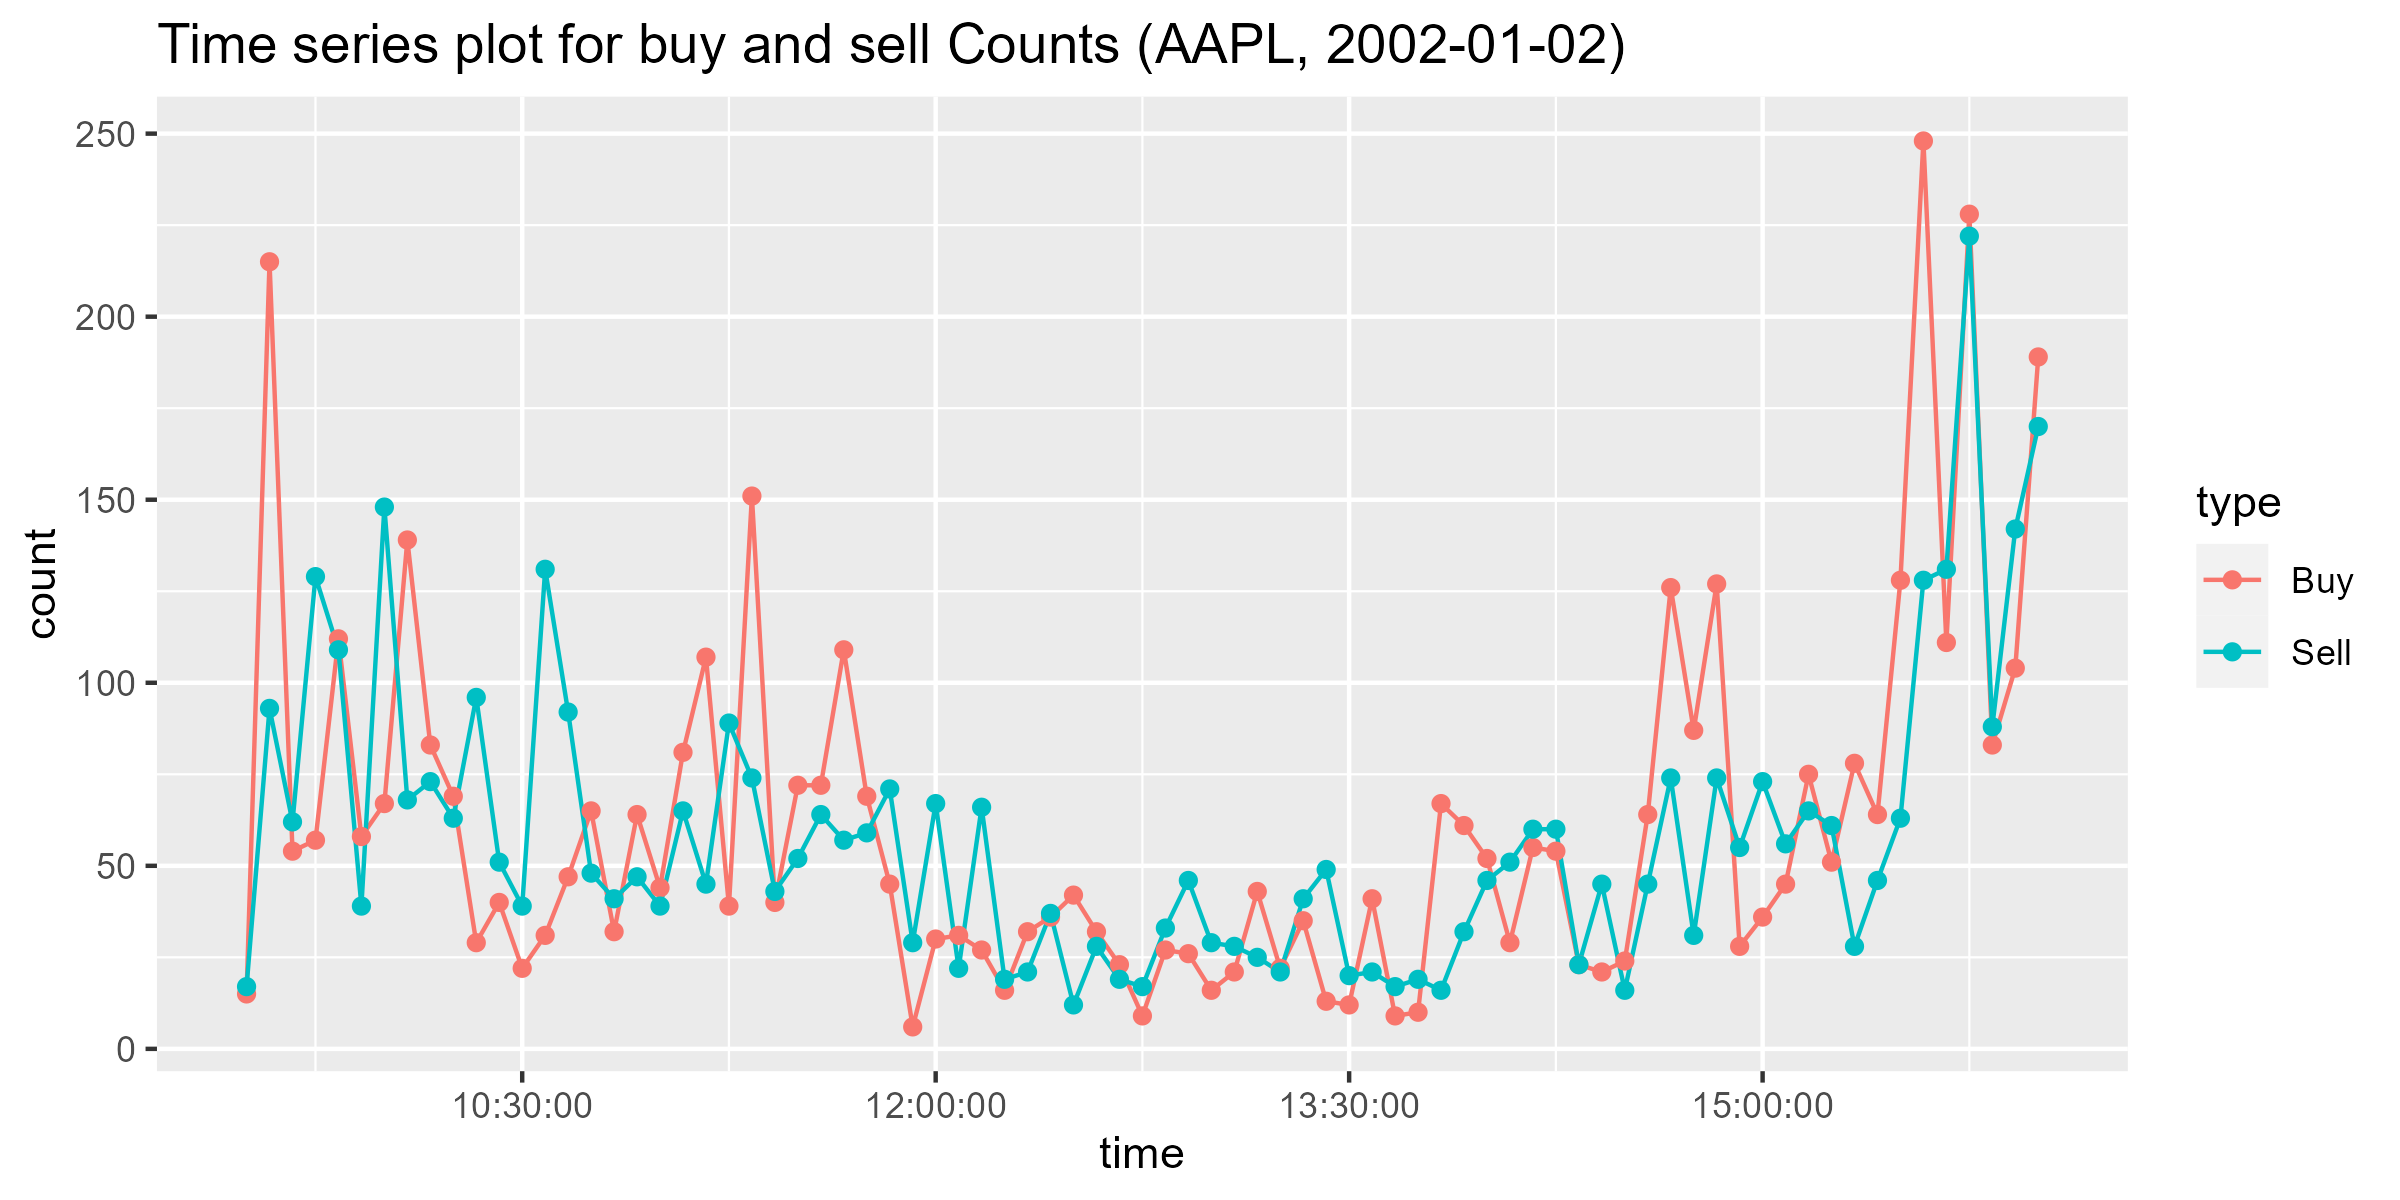
\includegraphics[width=\textwidth]{figures/TS(AAPL, 2002-01-02).png}
        \caption{Time series plot for buy and sell counts (AAPL, 2002-01-02)}
        \label{TS_AAPL}
    \end{figure}
\end{frame}

\begin{frame}{Introduction}
    \begin{figure}
        \centering
        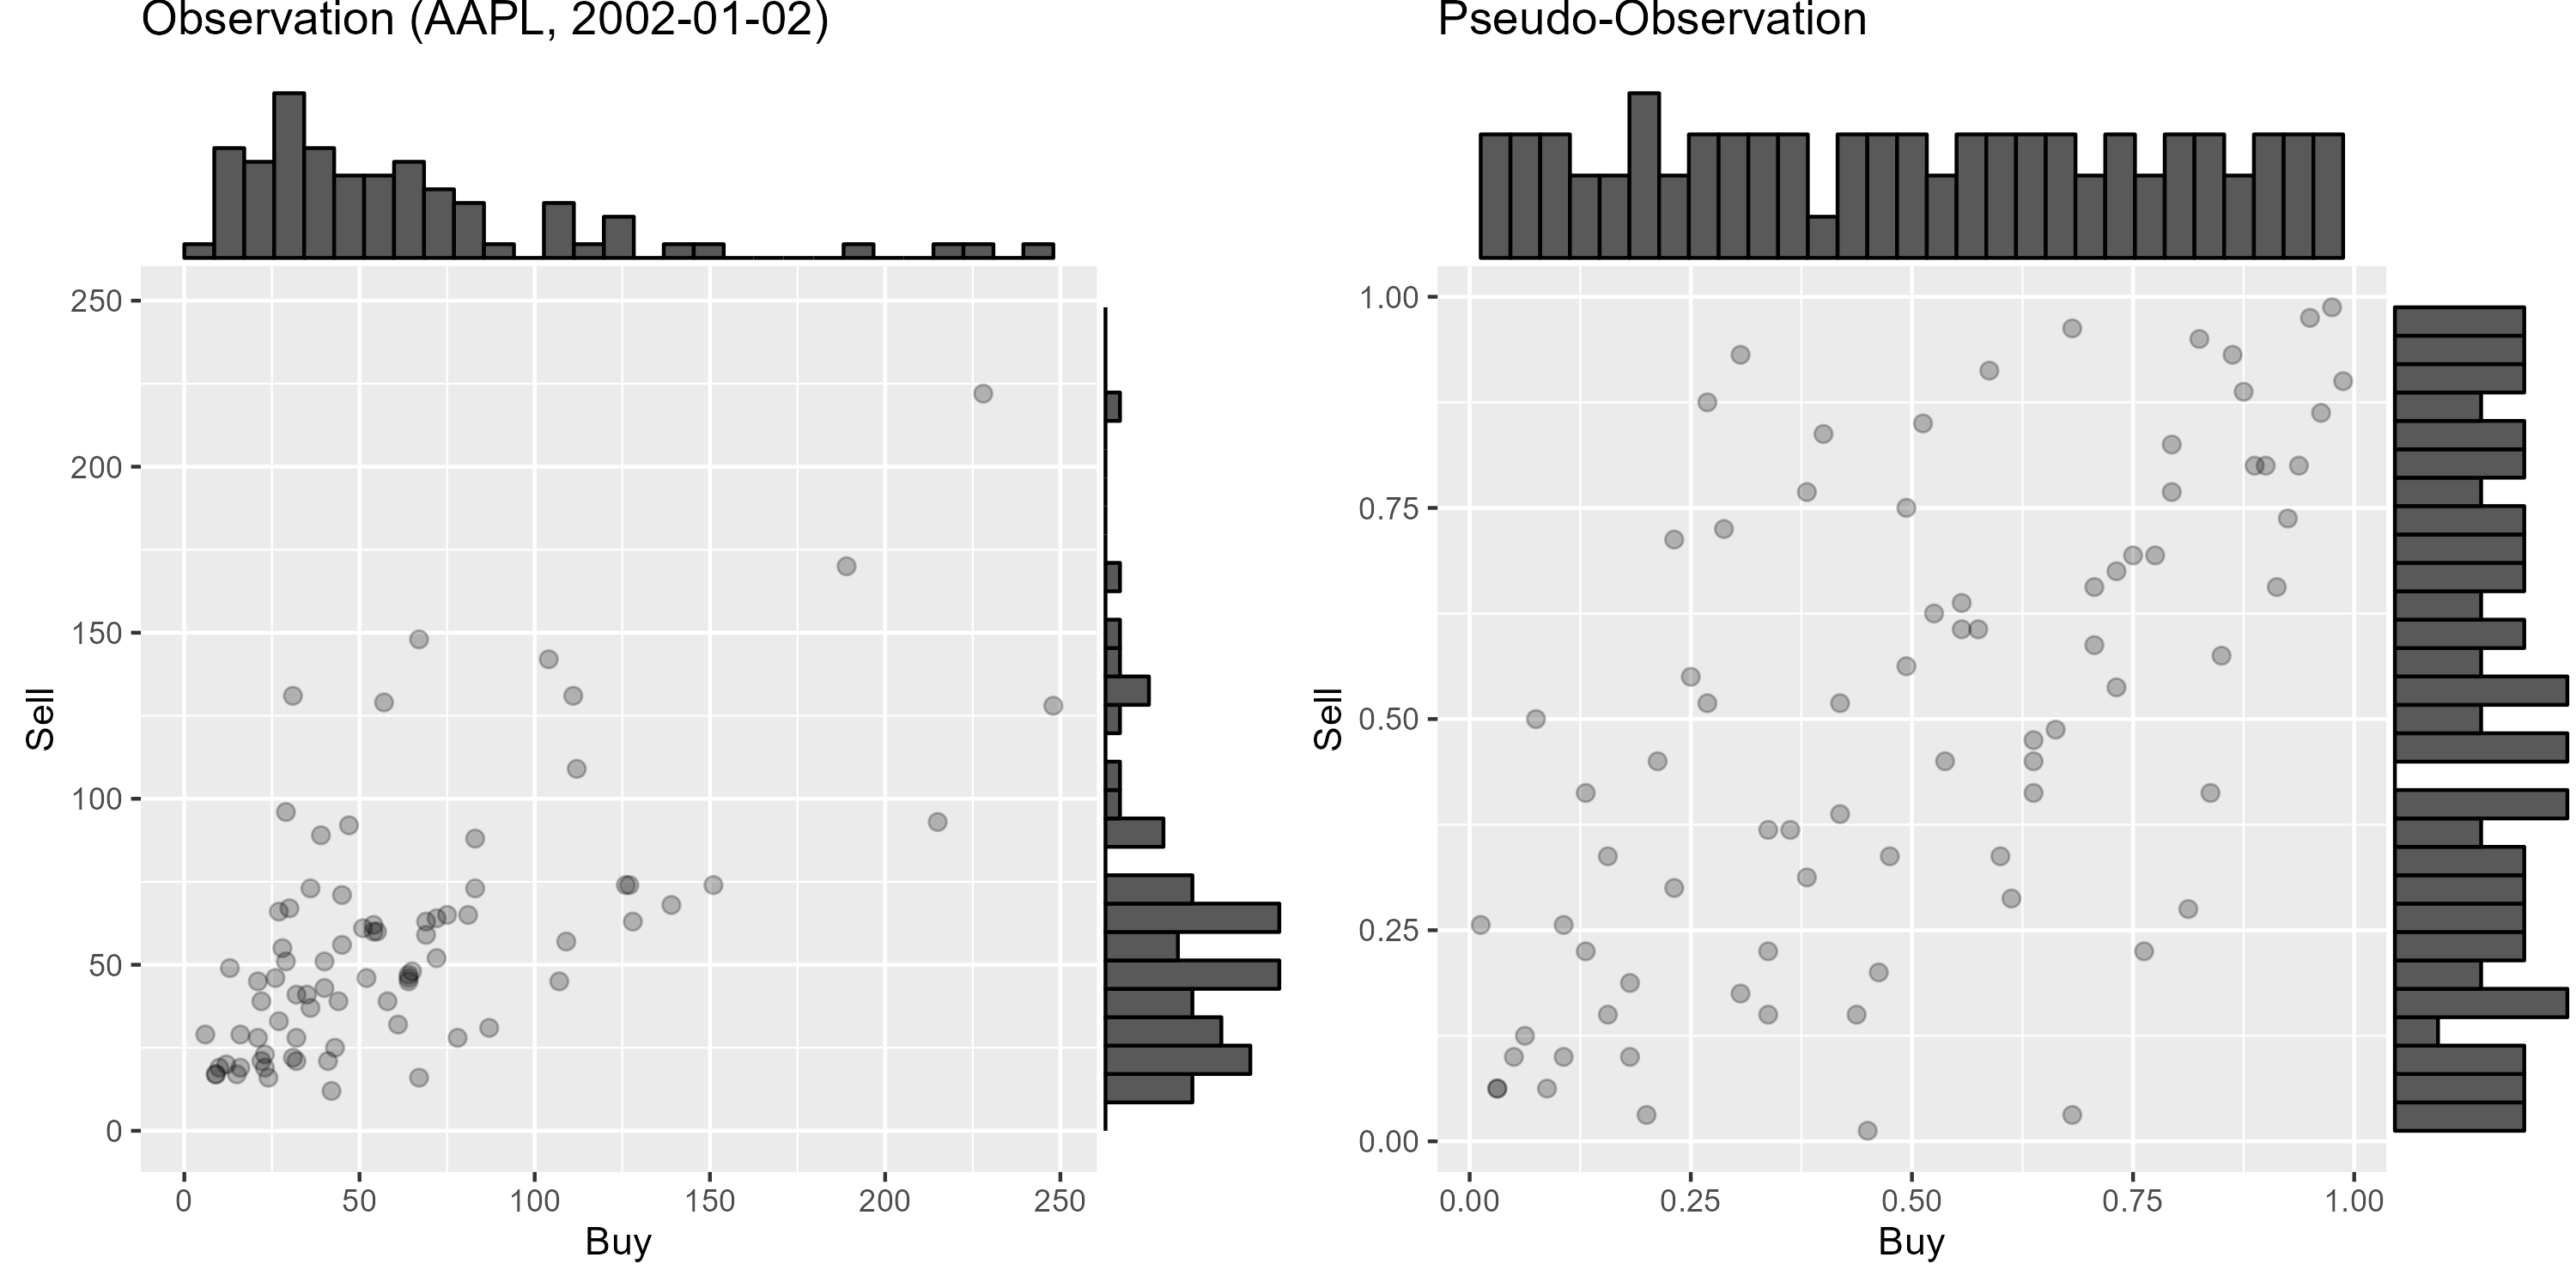
\includegraphics[width=\textwidth]{figures/Scatter(AAPL, 2002-01-02).png}
        \caption{The scatter plot for buy and sell counts (AAPL, 2002-01-02)}
        \label{SC_AAPL}
    \end{figure}
    Q: How to evaluate the PIN model with the {\color{red}correlation} structure?
\end{frame}


\section{Method}

\subsection{Copula}

\begin{frame}{Copula : Sklar's theorem}
    \begin{itemize}
        \item A \textcolor{red}{copula} is a multivariate cumulative distribution function with uniform marginal p.d.f of each variable is on $[0,1]$.

        \item Copulas allow us to model marginal distribution and joint relationships separately.
    \end{itemize}

    \begin{block}{Sklar's theorem}
        Every multivariate c.d.f. $H$ can be expressed in terms of its marginals $F_i$'s and a copula function $C$. \\
        \smallskip
        
        If the copula function has parameters $\theta \in \Theta$, and the marginal c.d.f. $F_i$ have parameters $\gamma_i \in \Gamma_i$,then 
        \begin{align*}
            H(\mathbf{x};\theta,\gamma) = C_\theta(F_1(x_1;\gamma_1),\cdots,F_p(x_p;\gamma_p)),
        \end{align*}
        where $\mathbf{x}=(x_1,\cdots,x_p)$
    \end{block}
\end{frame}

\begin{frame}{Example of copula}
    Some examples of copula :
    \begin{enumerate}
        \item Normal copula
        \small \begin{equation*}
            C^{(N)}_R(u_1,\cdots,u_p) = \Phi_R\left(\Phi^{-1}(u_1), \cdots, \Phi^{-1}(u_p) \right),
        \end{equation*}
        where $R$ is a correlation matrix
    
    \item Gumbel copula
        \small \begin{equation*}
            C^{(G)}_\theta(u_1,\cdots,u_p) = \exp\left[ -\left( \sum_i(-\log u_i)^\theta \right)^{1/\theta} \right], \theta\in[1,\infty)
        \end{equation*}

    \item Clayton copula
        \small \begin{align*}
            C^{(C)}_\theta(u_1,\cdots,u_p) = \left[ \max\left\{ \sum_i (u_i^{-\theta} -1) +1, 0 \right\} \right]^{-1/\theta}, 
        \end{align*}
        where $\theta\in[-1,\infty)\backslash\{0\}$

    \item Independent copula
        \small \begin{equation*}
            C^{(I)}(u_1,\cdots,u_p) = u_1 \cdots u_p
        \end{equation*}
    \end{enumerate}
\end{frame}

\begin{frame}{co-PIN model}
    The following is the structure of the co-PIN model : 
    \begin{figure}
        \centering
        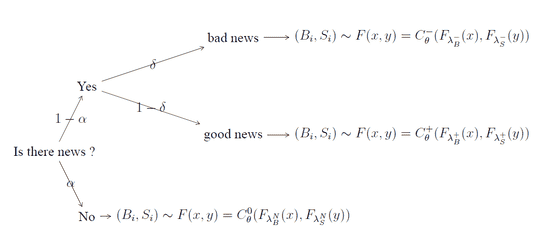
\includegraphics[width=\textwidth]{figures/CoPIN.png}
        \caption{The structure of the co-PIN model}
        \label{coPIN}
    \end{figure}
\end{frame}


\begin{frame}{Density express by copula}
    \begin{itemize}
        \item If marginals $F_j$ are continuous, and the density of copula exists, then the multivariate p.d.f. $h$ is given by
        \begin{equation*}
            h(\mathbf{x};\theta,\gamma) = c_\theta(F_1(x_1;\gamma_1),\cdots,F_p(x_p;\gamma_p)) \prod_{t=1}^p f_t(x_t;\gamma_t),
        \end{equation*}
        where $c_\theta(u_1,\cdots,u_p)=\frac{\partial^p C_\theta(u_1,\cdots,u_p)}{\partial u_1 \cdots \partial u_p}$ is the density of the copula.

        \item For the discrete marginal, we can express $h$ as the following
        \begin{align*}
            h(\mathbf{x};\theta,\gamma) &= \sum_{i_1=0}^1 \cdots \sum_{i_p=0}^1 (-1)^{i_1+\cdots+i_p} \\
            &\times C_\theta(F_1(x_1-i_1;\gamma_1),\cdots,F_p(x_p-i_p;\gamma_p))
        \end{align*}
    \end{itemize}
\end{frame}


\subsection{ECM algorithm}

\begin{frame}{ECM algorithm}
    The expectation conditional maximization (ECM) algorithm is the variants of the EM algorithm, which separate the M-step into a sequence of conditional maximization (CM) steps.\\
    \bigskip
    Let $\psi=(\theta,\gamma) \in \Theta \times \Gamma$. Divide the M-step into 2 CM-steps :
    \begin{enumerate}
        \item CM-step1 (maximize w.r.t. $\gamma$) :
        \begin{equation*}
            \gamma^{(l+1)} = \argmax_\Gamma \sum_{j=1}^m \sum_{i=1}^n w_{ij}^{(l+1)} \log h_j(\mathbf{x}_i;\theta_j^{(l)},\gamma_j).
        \end{equation*}

        \item CM-step2 (maximize w.r.t. $\theta$) :
        \begin{equation*}
            \theta^{(l+1)} = \argmax_\Theta \sum_{j=1}^m \sum_{i=1}^n w_{ij}^{(l+1)} \log h_j(\mathbf{x}_i;\theta_j,\gamma_j^{(l+1)}).
        \end{equation*}
    \end{enumerate}
\end{frame}


\begin{frame}{ECM algorithm}
    \begin{enumerate}
        \item E-step: Calculate
        $\displaystyle w_{ij}^{(l+1)} = \frac{\pi_j^{(l)} h_j(\mathbf{x}_i;\psi_j^{(l)})}{\sum_{j=1}^m \pi_j^{(l)} h_j(\mathbf{x}_i;\psi_j^{(l)})} \, (i=1,\cdots,n, \, j=1,\cdots,m)$
        
        \item M-step (for $j=1,\cdots,m$) \\
        \begin{enumerate}
            \item Set 
            $\displaystyle \pi_j^{(l+1)} = \frac{1}{n} \sum_{i=1}^n w_{ij}^{(l+1)}$

            \item CM-step1 : 
            $\displaystyle \gamma_j^{(l+1)} = \argmax_\Gamma \sum_{i=1}^n w_{ij}^{(l+1)} \log h_j(\mathbf{x}_i;\theta_j^{(l)},\gamma_j)$.

            \item CM-step2 :
            $\displaystyle \theta_j^{(l+1)} = \argmax_\Theta \sum_{i=1}^n w_{ij}^{(l+1)} \log h_j(\mathbf{x}_i;\theta_j,\gamma_j^{(l+1)})$
        \end{enumerate}

        \item Stop if $\left\| \ell \left(\mathbf{x};\psi^{(l+1)},\pi^{(l+1)} \right) - \ell \left(\mathbf{x};\psi^{(l)},\pi^{(l)} \right) \right\| < \varepsilon$
    \end{enumerate}
\end{frame}


\section{Simulation study}

\begin{frame}{Simulation}
    \begin{enumerate}
        \item Generate datasets with 500 two-dimensional data points with 2 clusters and then fit the models.
        
        \item Construct the data from specified marginals (Poisson) and copulas (normal, Gumbel, Clayton), then fit the simulation data with the same model setting. 
        
        \item Repeat 1000 times, Check the difference with a histogram, and scatter plot of error rates vs. distances between two clusters.

        \item To compare different copulas parameters, we use the association measure Kendall's tau,
        \begin{equation*}
            \tau(X_1,X_2) = 4\iint_{[0,1]^2} C(u,v) \, dC(u,v) -1
        \end{equation*}
    \end{enumerate}
\end{frame}

\begin{frame}{Simulation}
    \begin{figure}
        \centering
        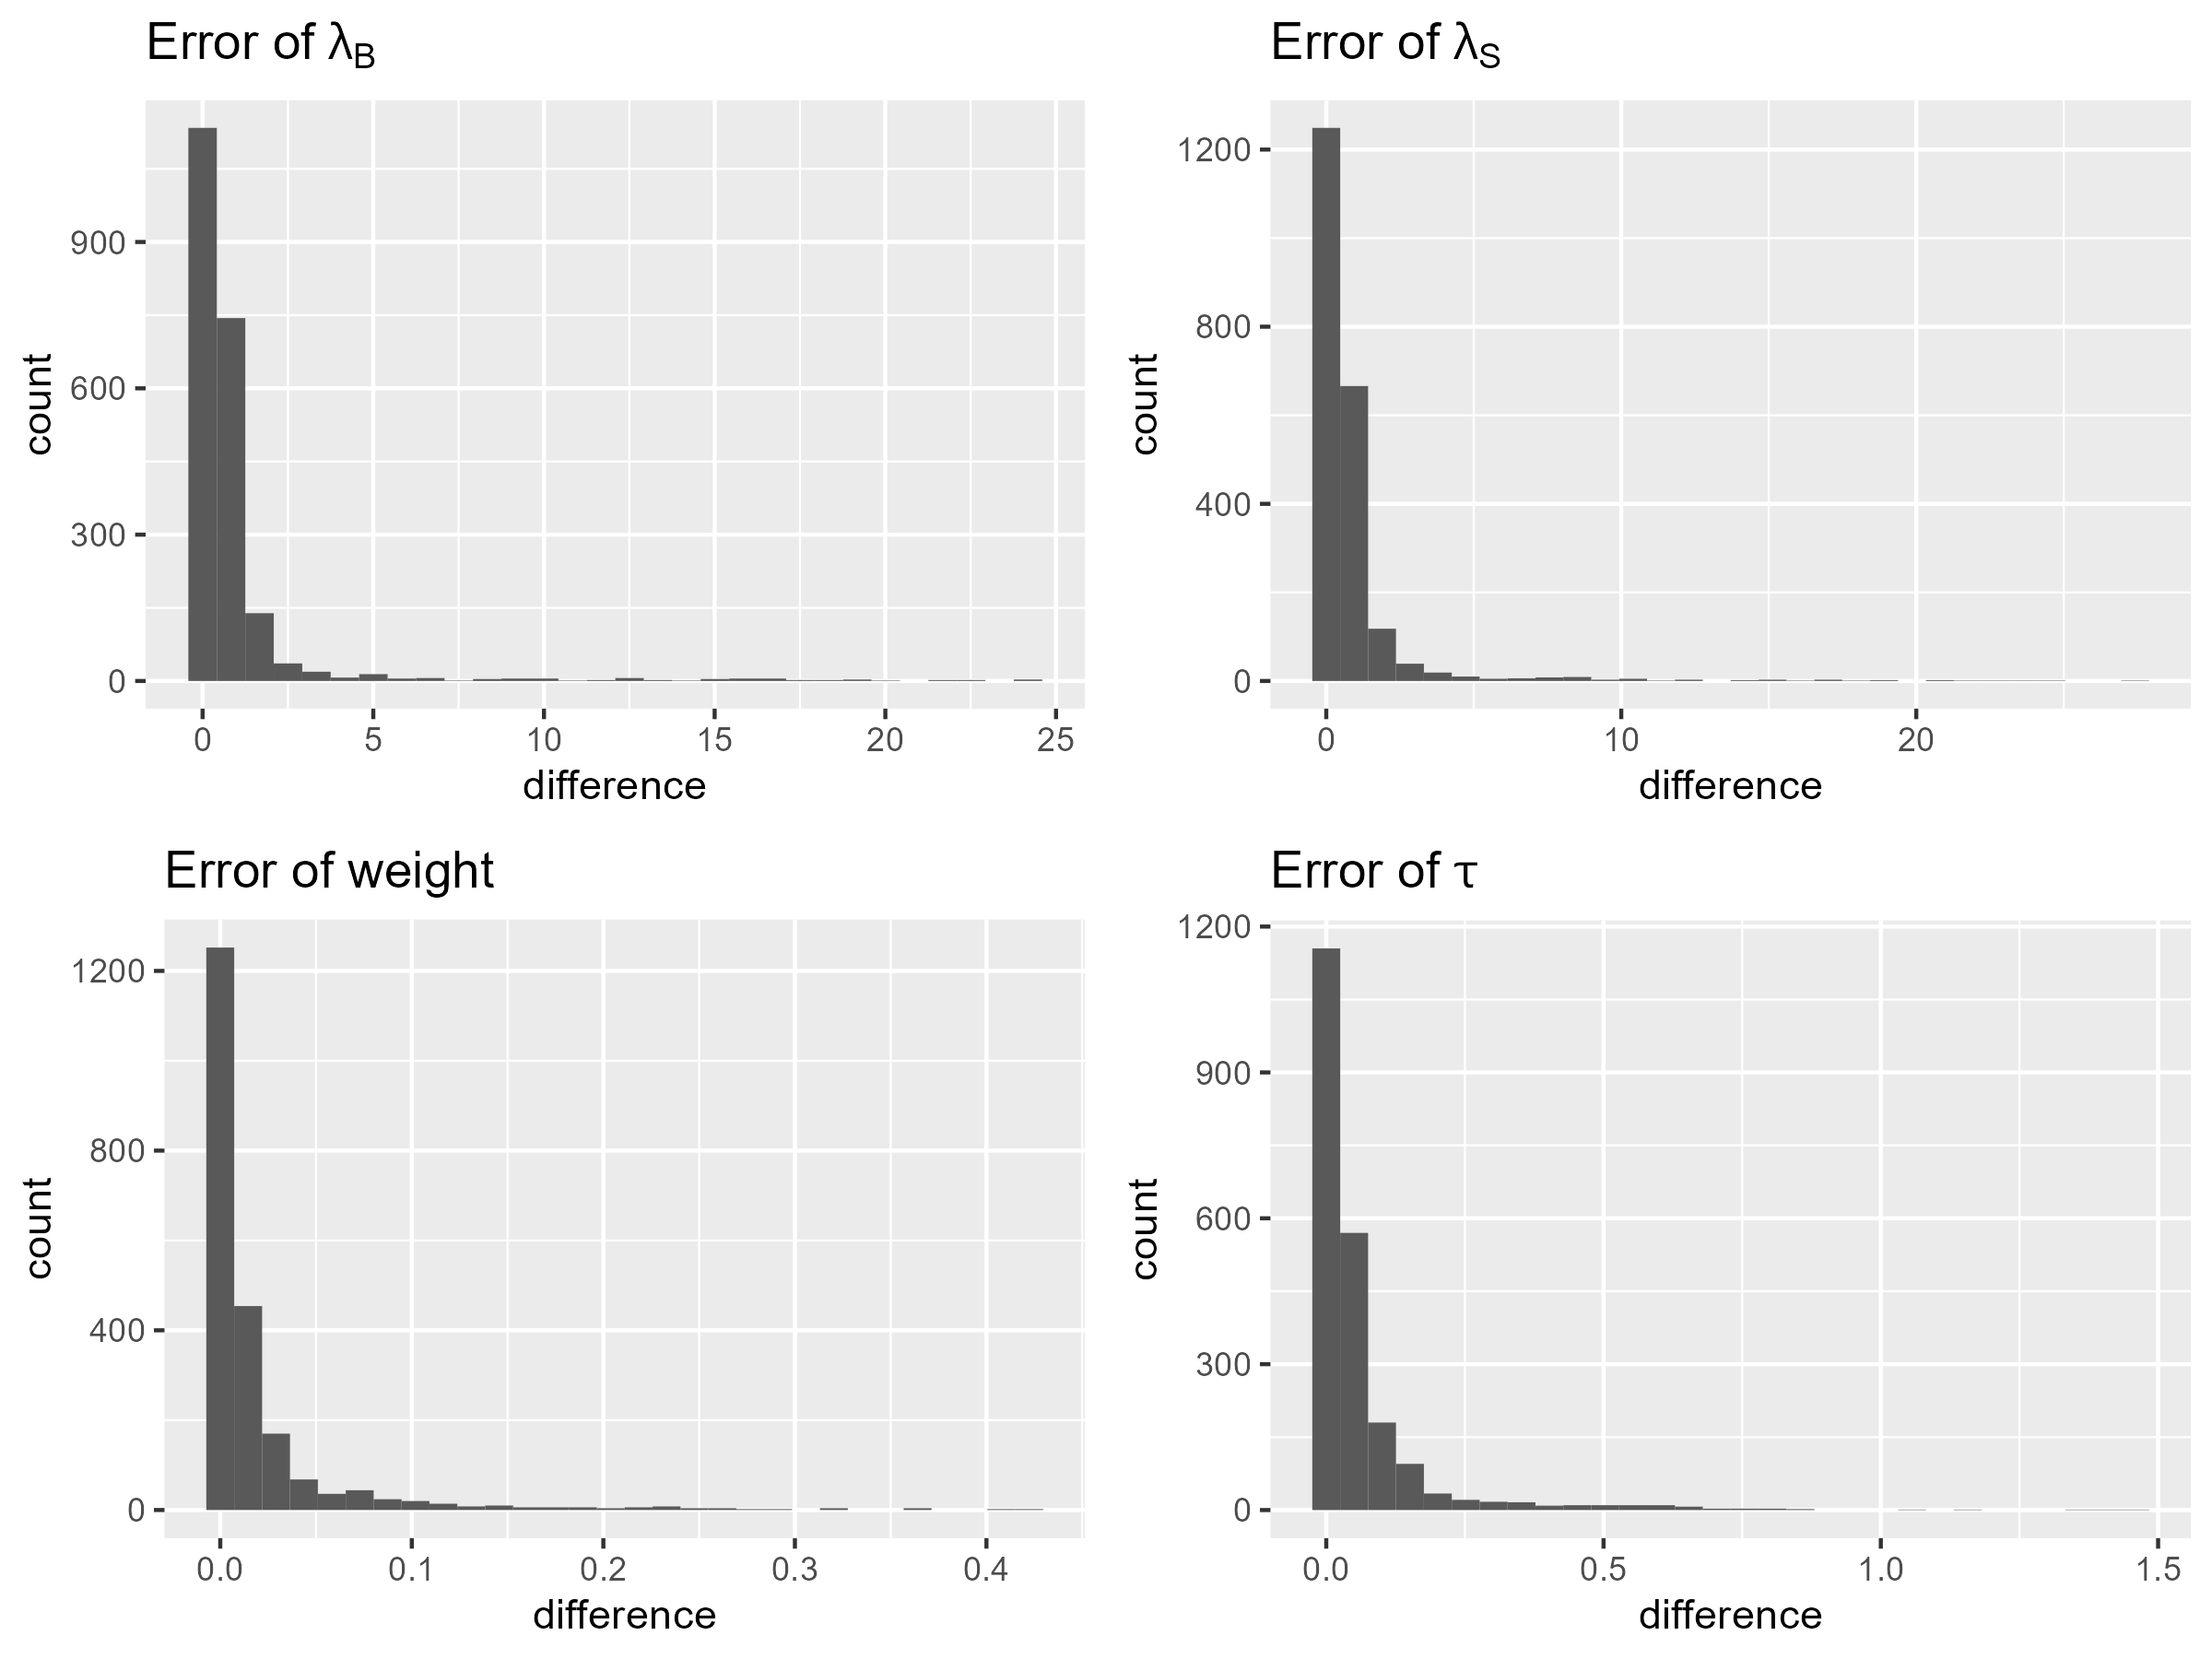
\includegraphics[width=8.5cm]{figures/Err.png}
        \caption{Histogram of absolute error of parameters}
        \label{err}
    \end{figure}
\end{frame}

\begin{frame}{Simulation}
    \begin{figure}
        \centering
        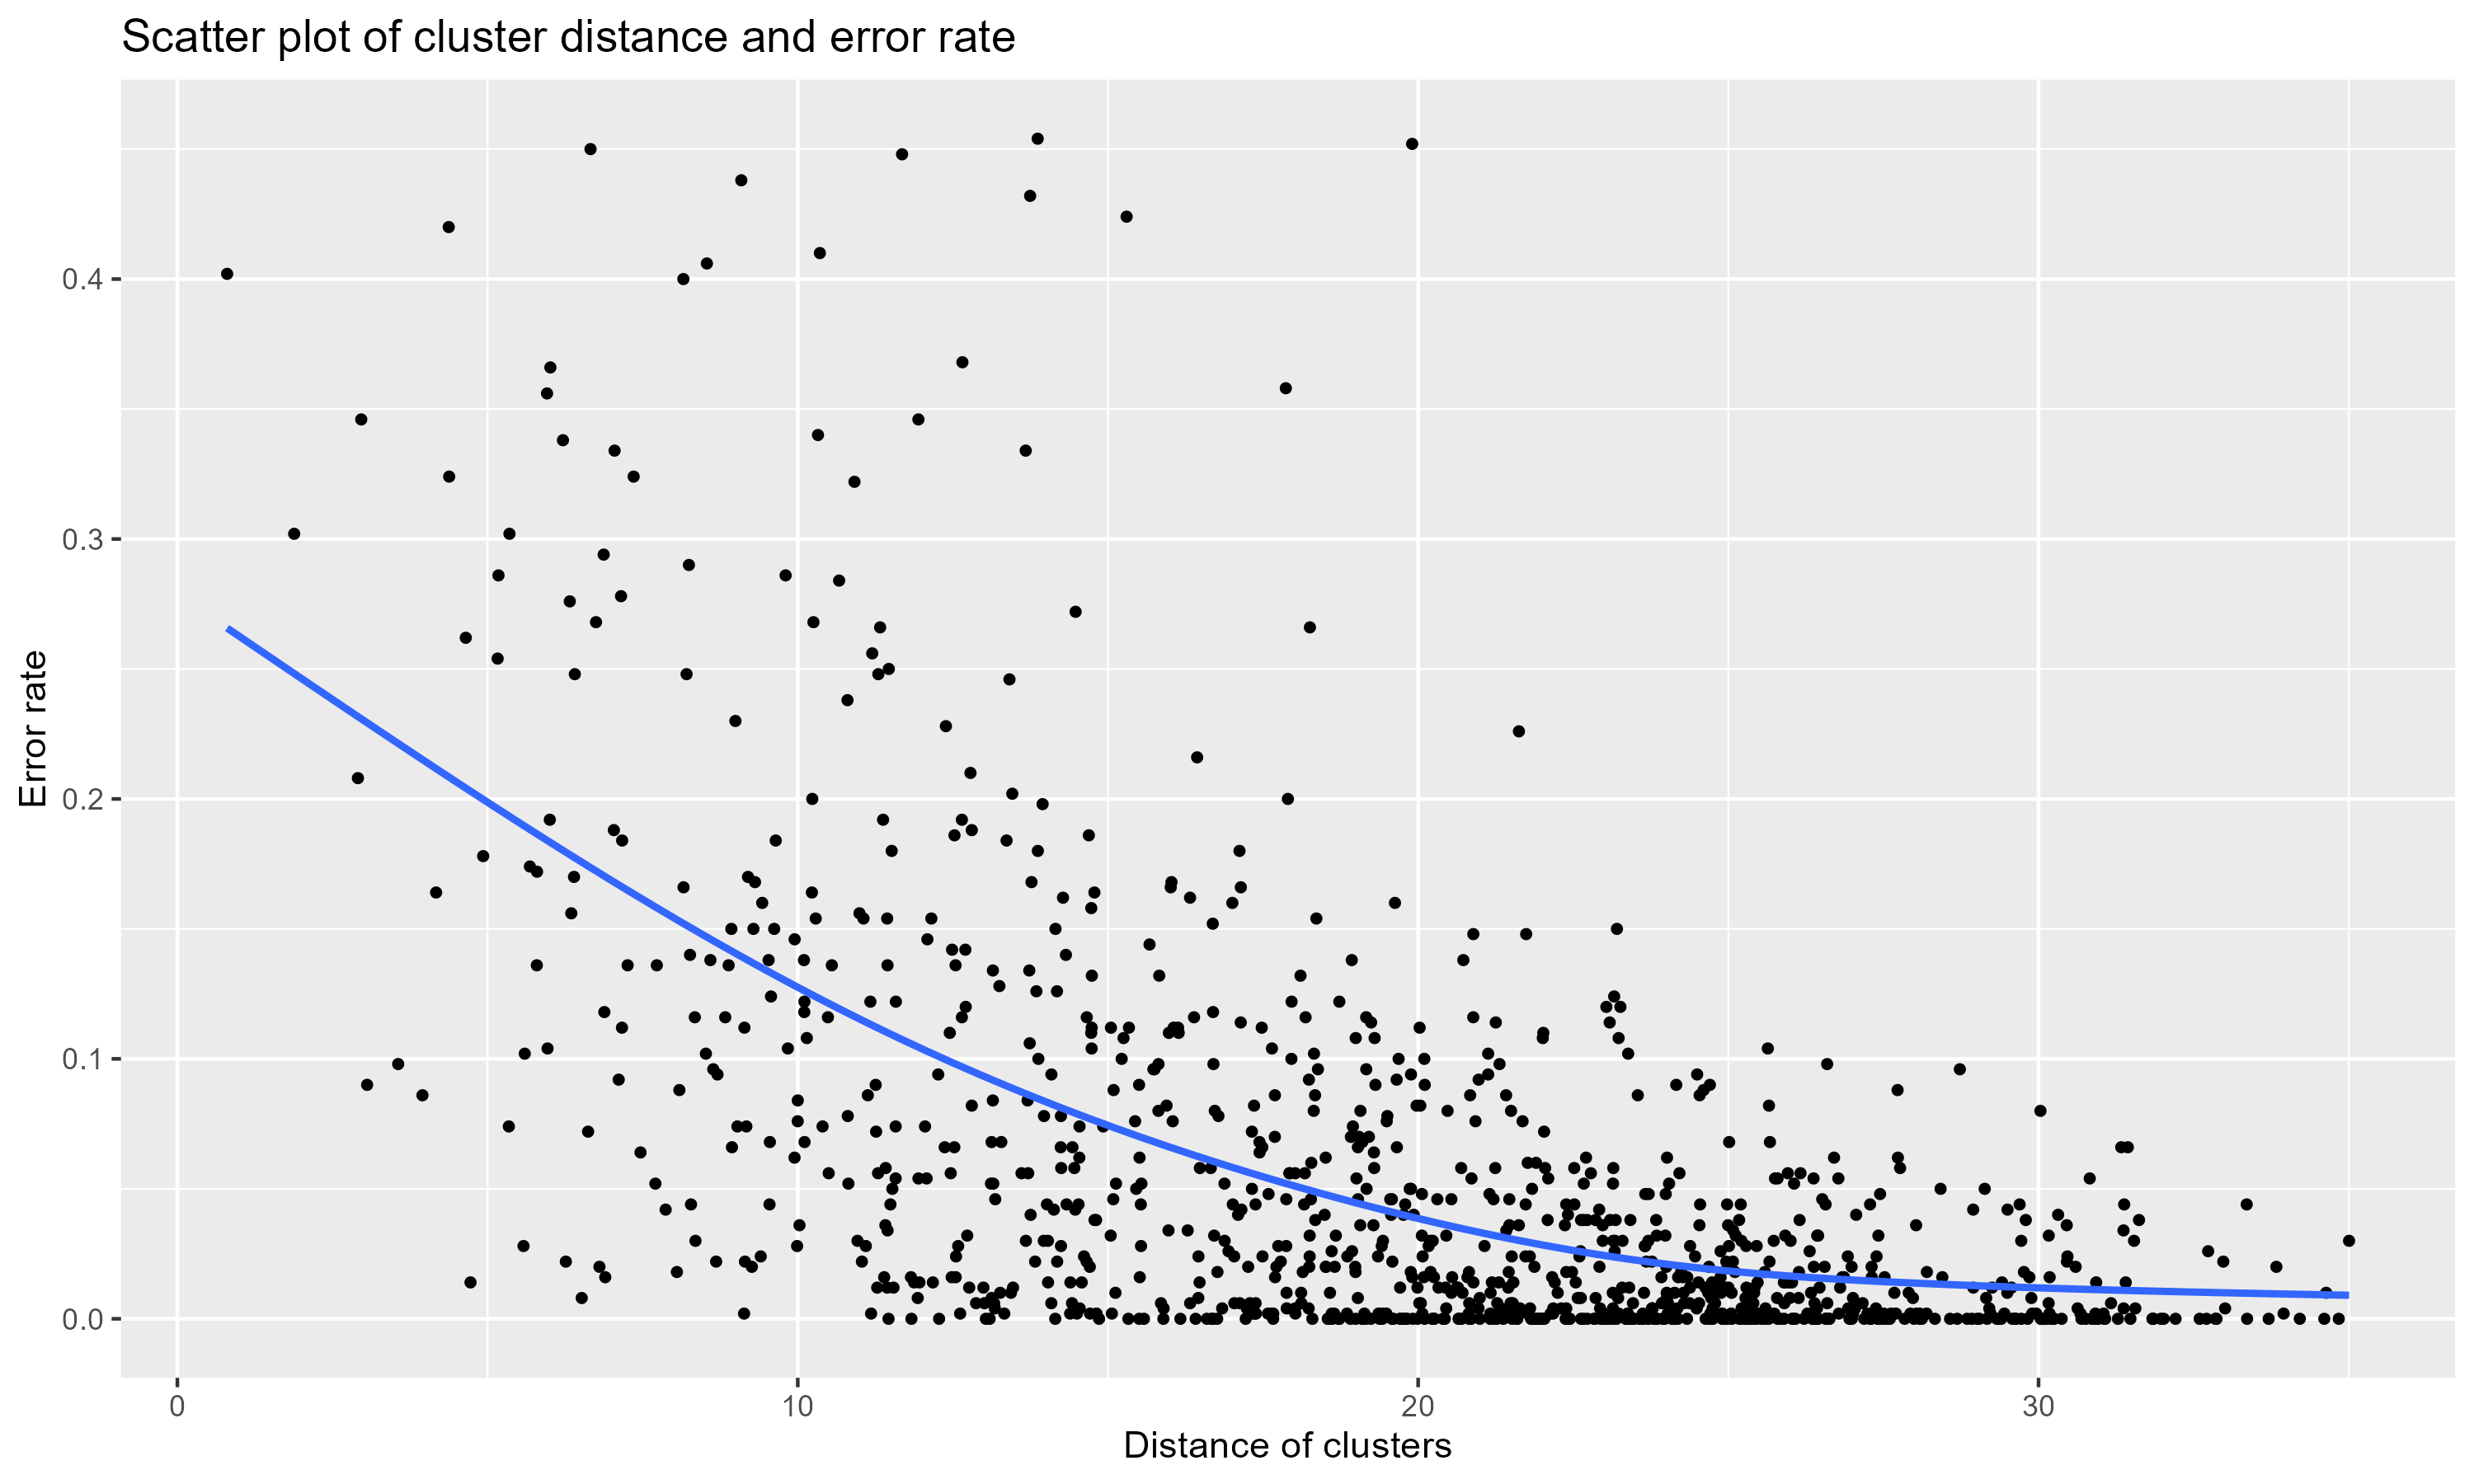
\includegraphics[width=\textwidth]{figures/err_dis.png}
        \caption{Scatter plot of classification error rate vs. cluster distance}
        \label{err_dis}
    \end{figure}
\end{frame}

\section{Real data analysis}

\begin{frame}{Real data analysis}
    \begin{itemize}
        \item Use the daily trading records of AAPL (large) and NTE (small) stocks in 2008, which were collected every 5 minutes. We only use data within U.S. stock market trading hours, resulting in about 249 days, and 78 data points per day.

        \item Using zero-inflated Poisson (ZIP) for marginal may better fit the relatively small firm or short-term data.
        
        \item In the original PIN model, the point with $0$ mostly be in the cluster of ``no news". We think that $0$ could also represent news in the market, but traders tend not to trend. 
    \end{itemize}

    \begin{equation*}\label{pmf-ZIP}
        P\left\{ X = x \right\} =
        \begin{cases}
            \phi + (1-\phi) e^{-\lambda}, & x = 0, \\
            (1-\phi) \frac{\lambda^x e^{-\lambda}}{x!}, & x \geq 1,
        \end{cases}
    \end{equation*}
\end{frame}


\begin{frame}{Stock NTE in 2008}
    \begin{figure}
	   \begin{subfigure}{.49\textwidth}
	    \centering
        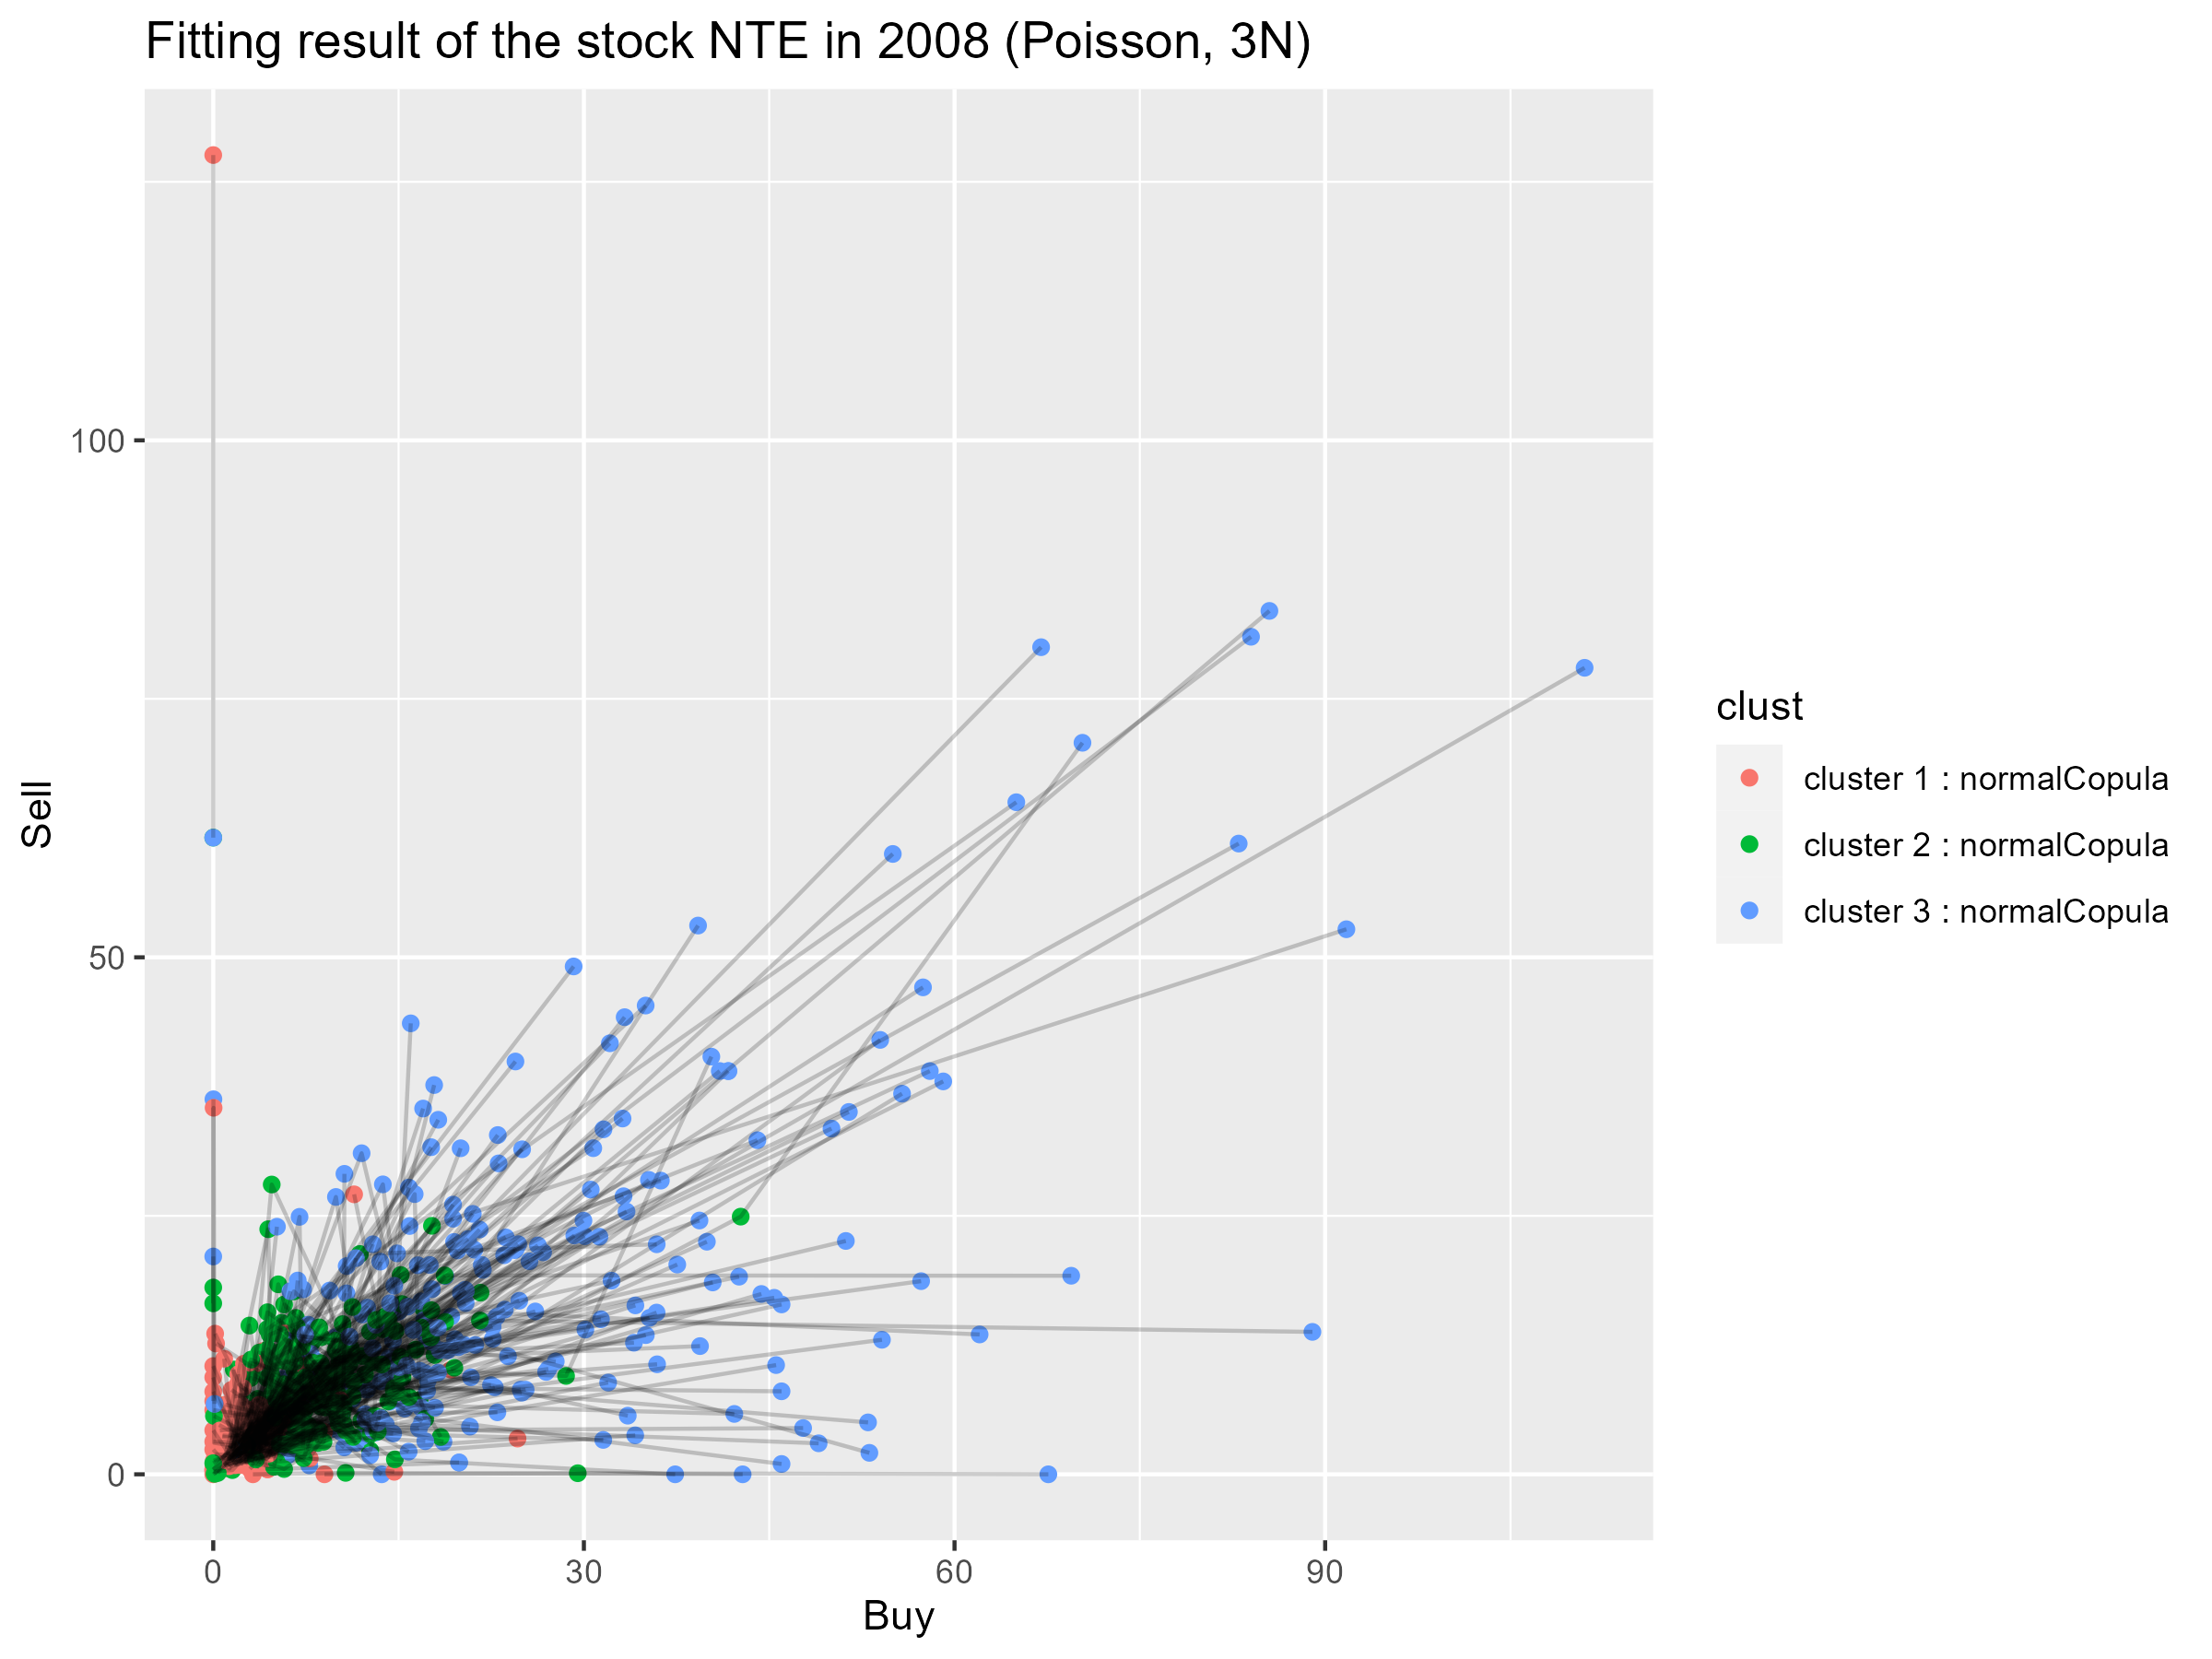
\includegraphics[width=\textwidth]{figures/fit_poi_NNN_NTE_2008_BS.png}
		\caption{3 Normal Copulas}\label{NNN_NTE_poi}
	   \end{subfigure}
	   \begin{subfigure}{.49\textwidth}
		\centering
        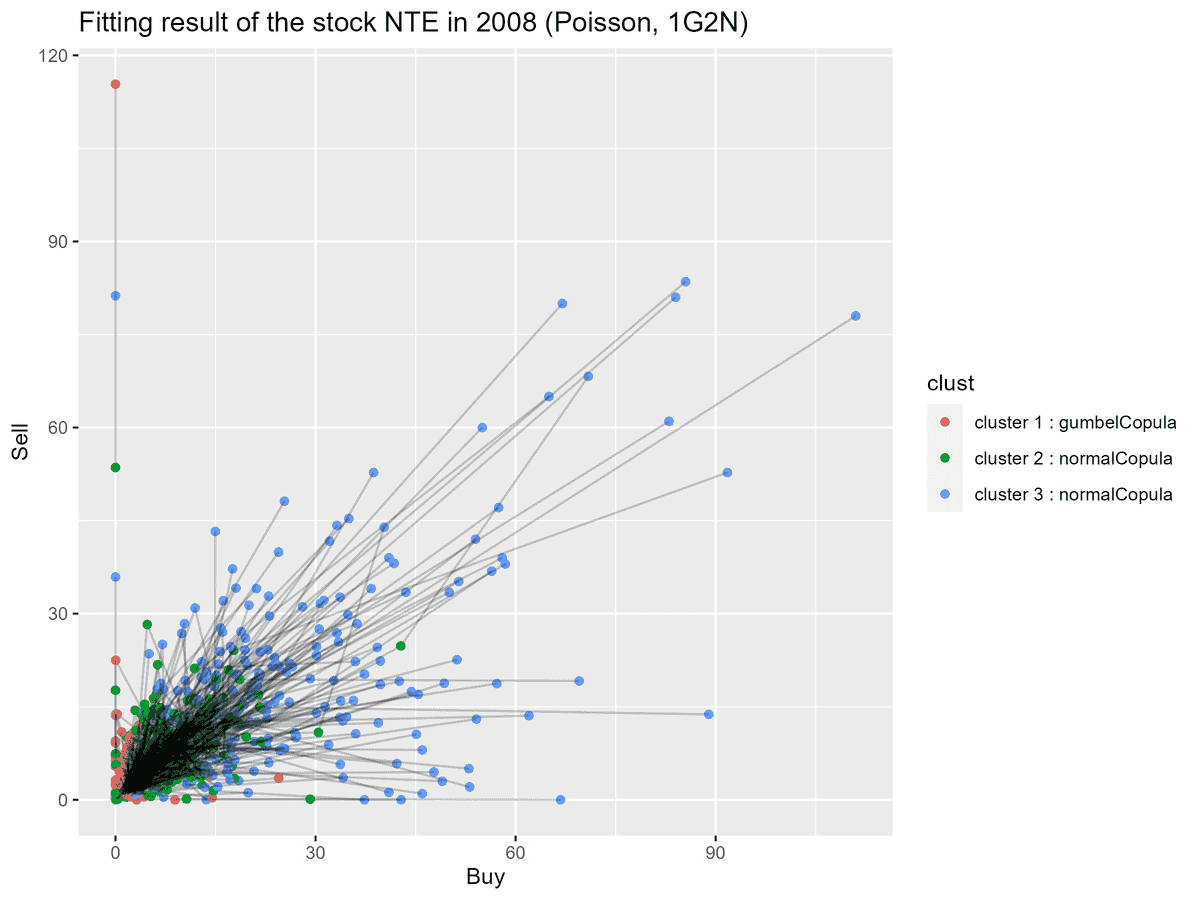
\includegraphics[width=\textwidth]{figures/fit_poi_GNN_NTE_2008_BS.png}
		\caption{1 Gumbel + 2 Normal Copulas}\label{GNN_NTE_poi}
	   \end{subfigure}
        \caption[Poisson rate of the NTE stock in 2008]{Poisson rate of the NTE stock in 2008 {under different copula combinations.} All lines connect 3 points of the fit in one day.}
        \label{poi_NTE_2008_BS}
    \end{figure}
\end{frame}

\begin{frame}{Stock NTE in 2008}
    \begin{figure}
        \centering
        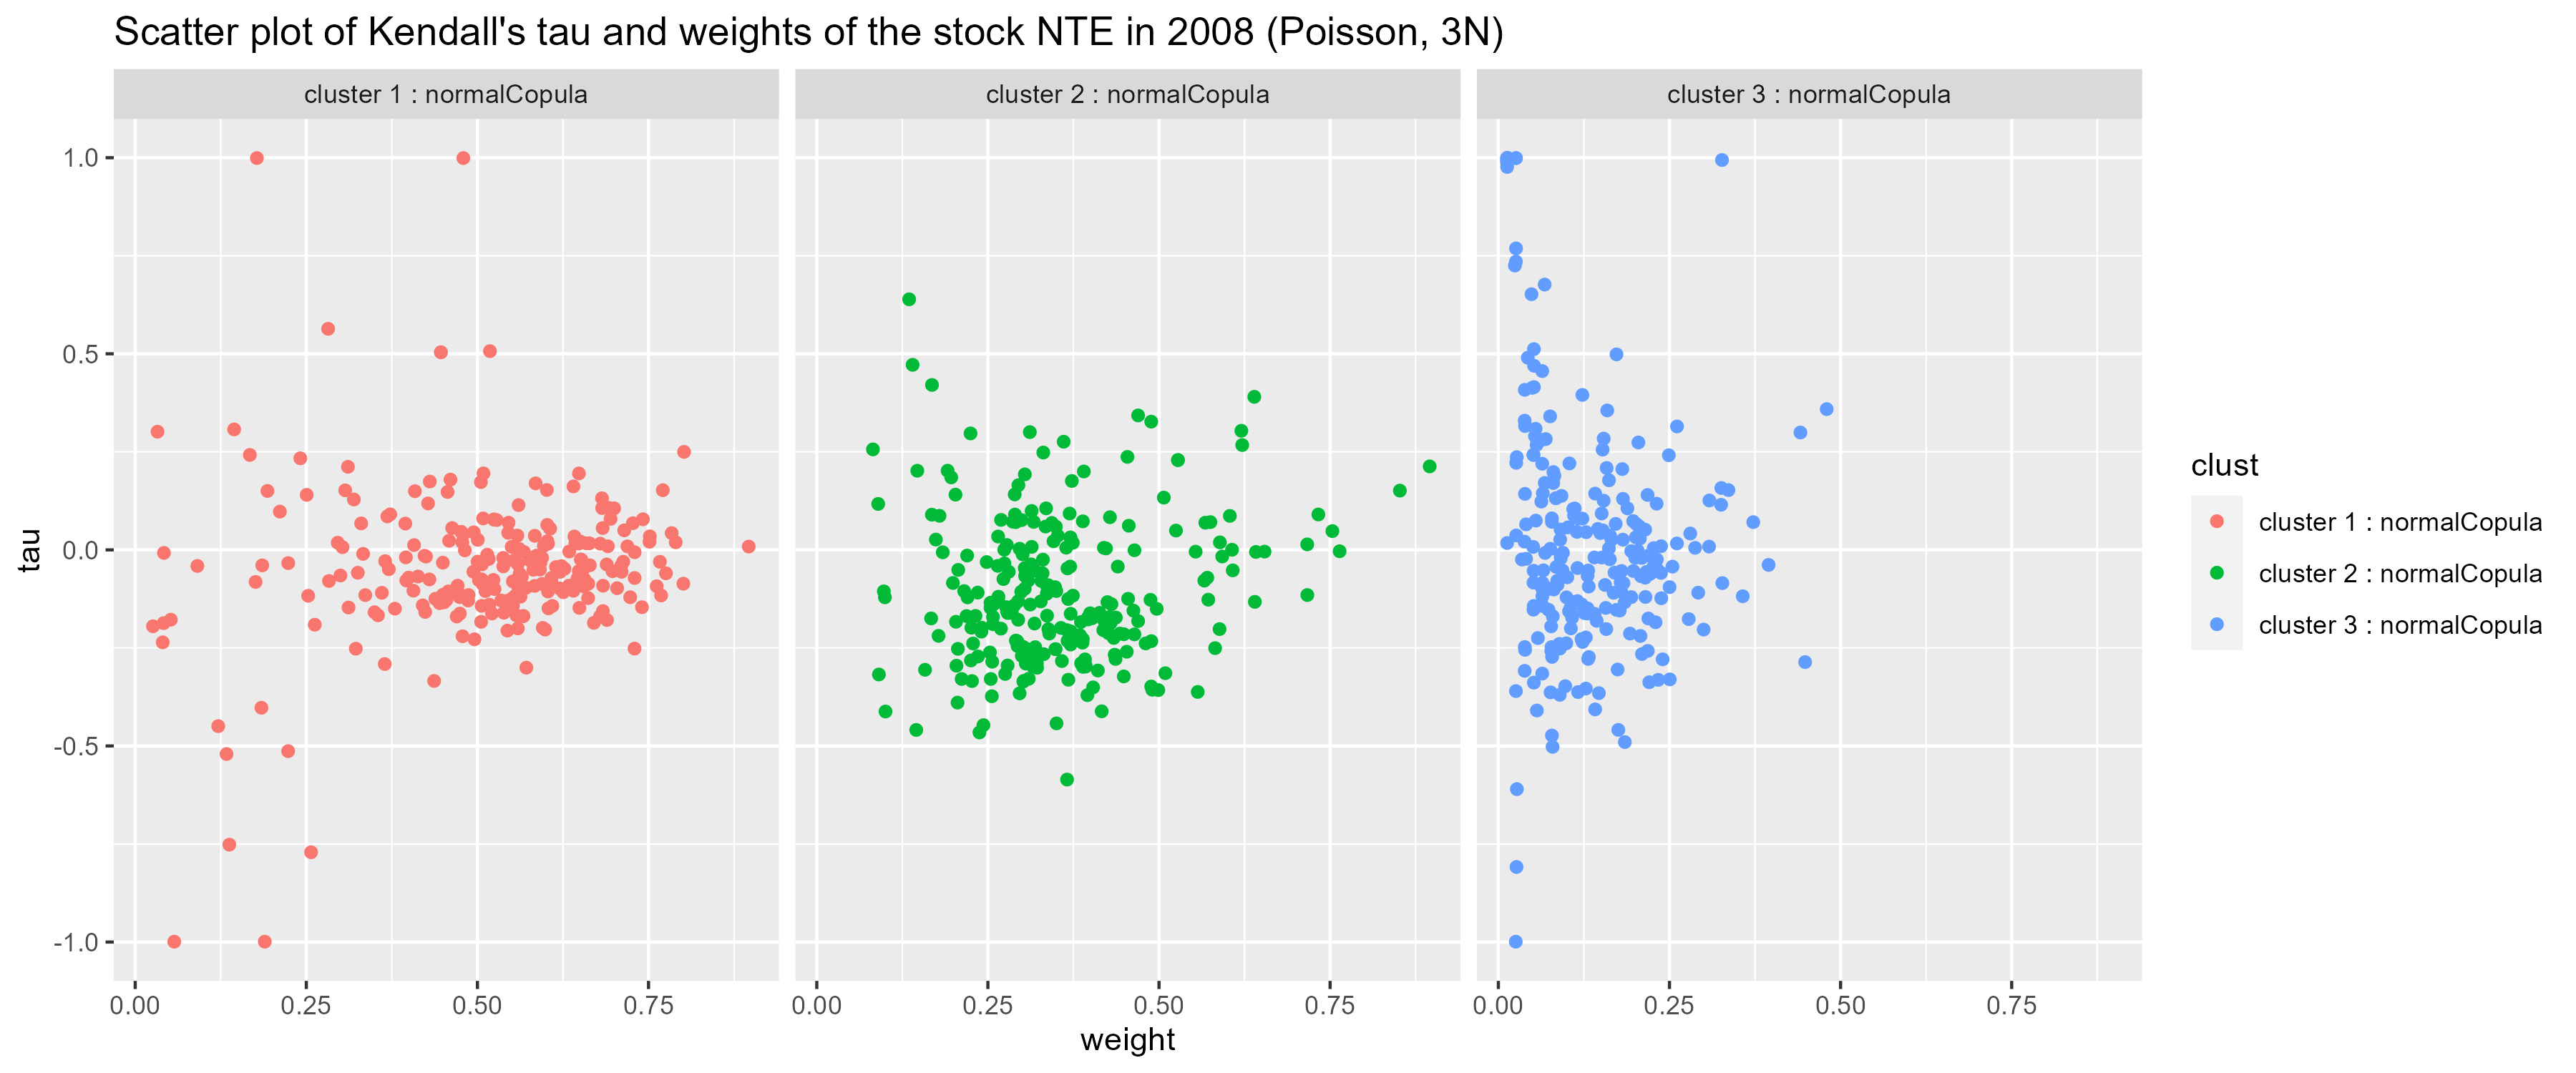
\includegraphics[width=\textwidth]{figures/fit_poi_NNN_NTE_2008_cw.png}
        \caption{Scatter plot of Kendall's tau and the weights of the NTE stock in 2008 (Poisson, 3 normal).}
    \label{poi_NNN_NTE_2008_cw}
    \end{figure}
\end{frame}


\begin{frame}{Stock NTE in 2008}
    \begin{figure}
        \centering
        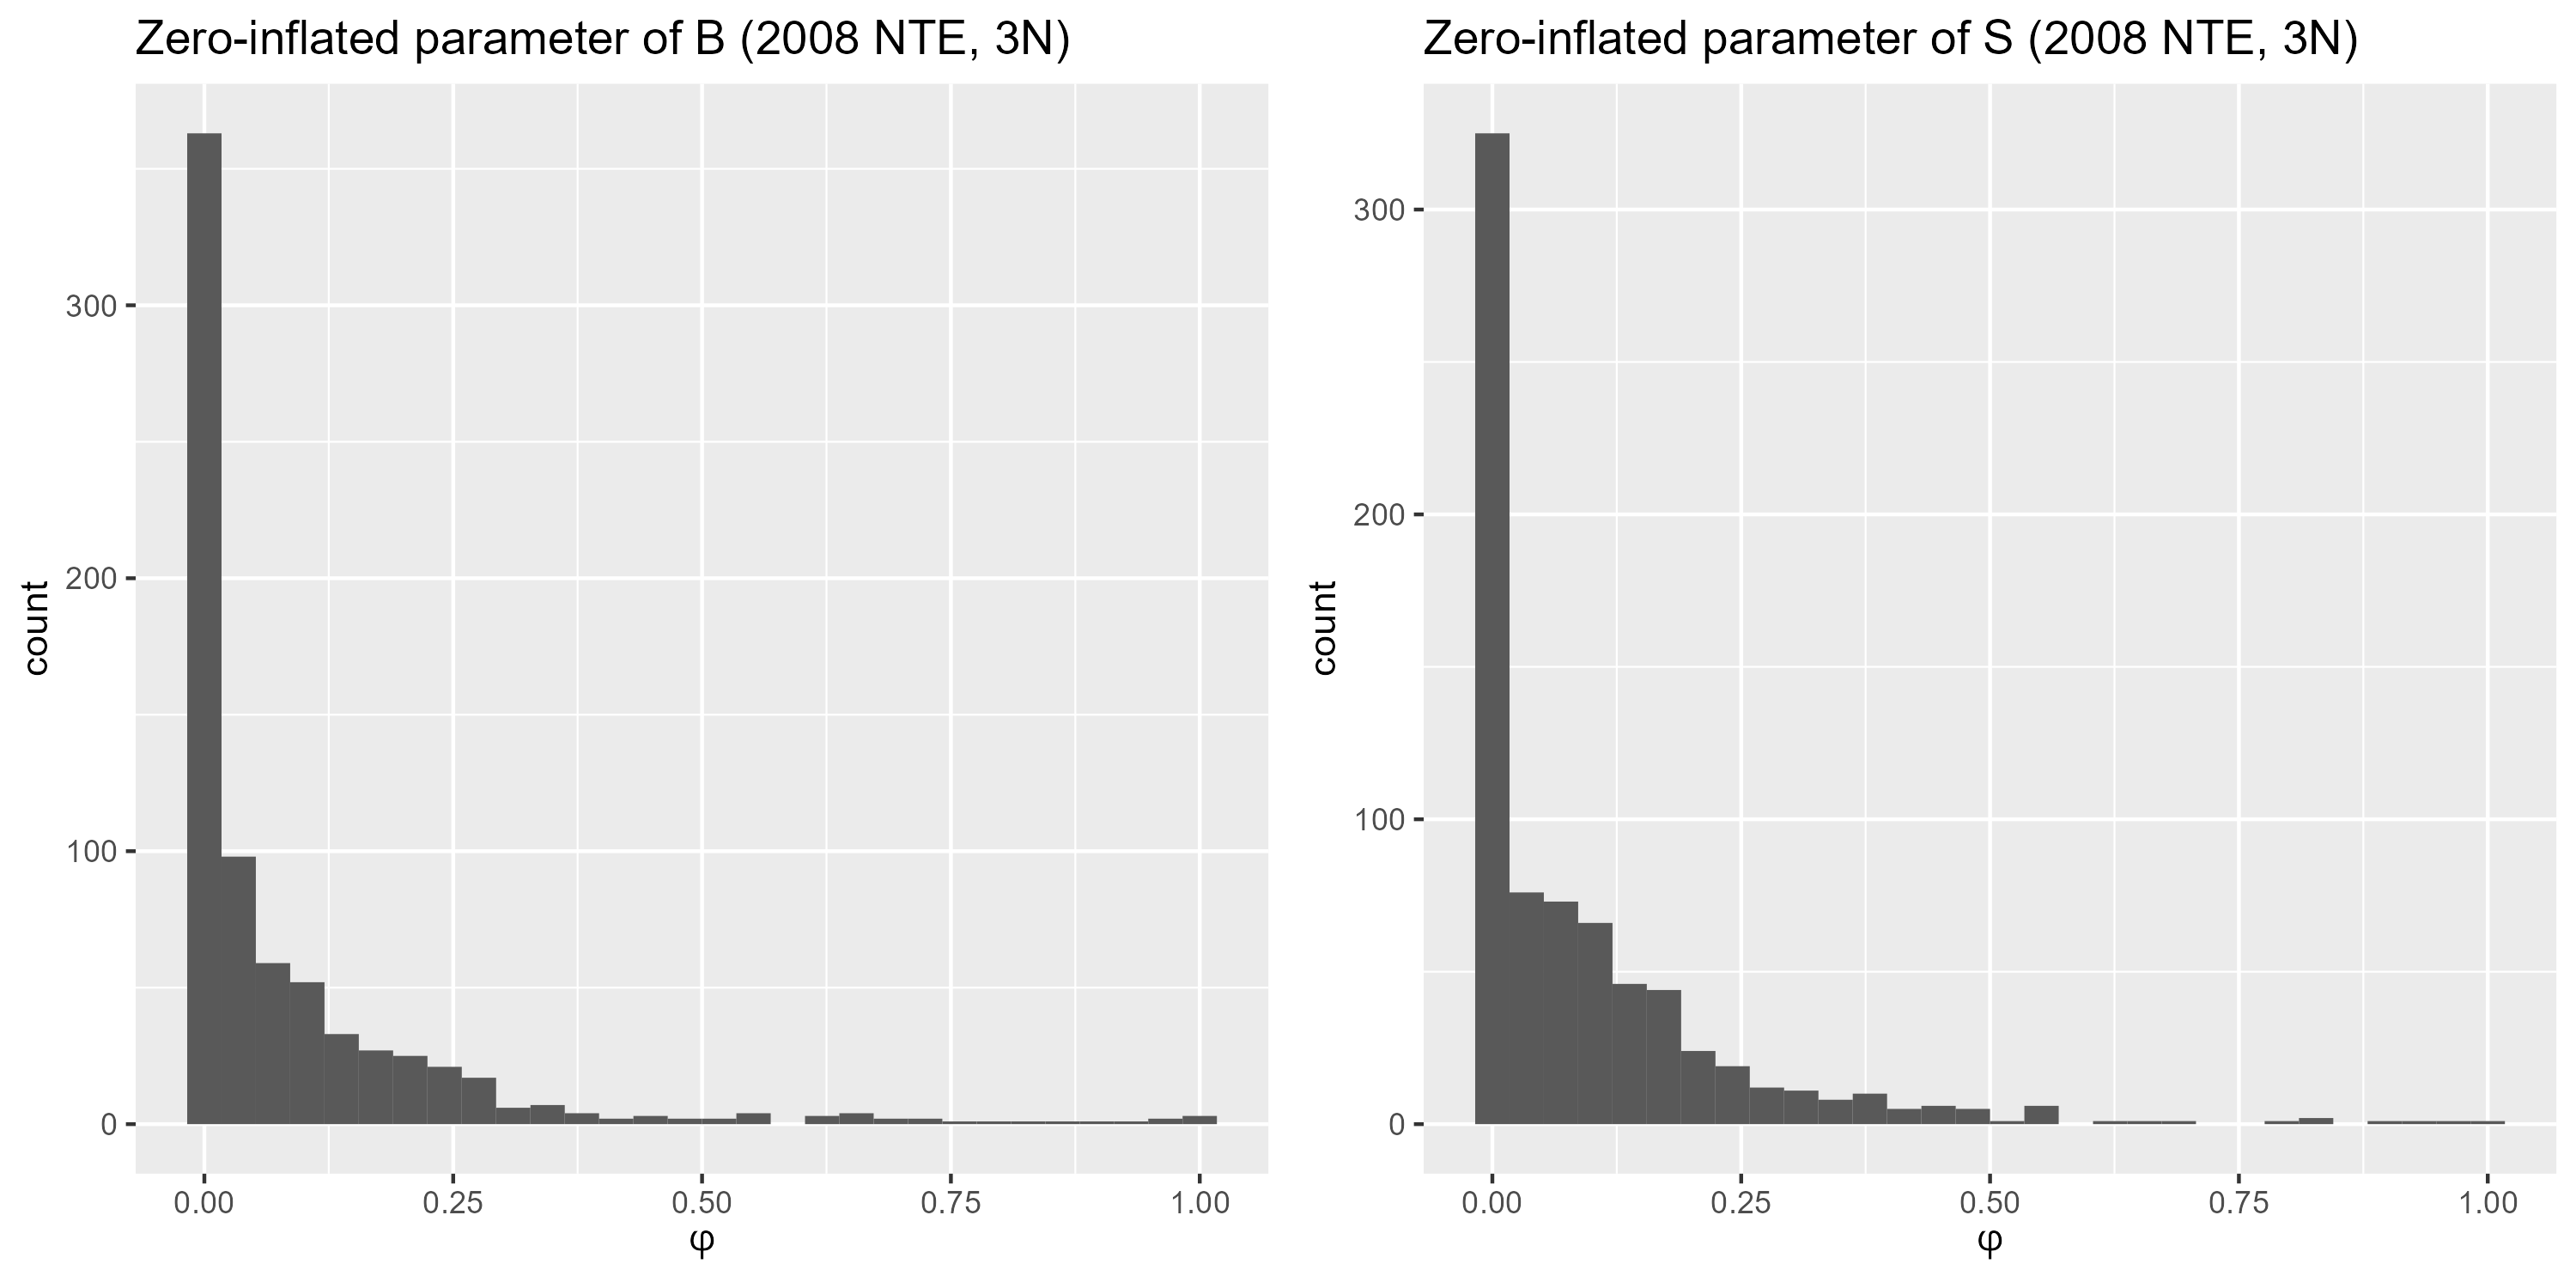
\includegraphics[width=\textwidth]{figures/fit_zip_NNN_NTE_2008_zi.png}
        \caption{Histogram of zero-inflated parameters of the NTE stock in 2008 (3N)}
        \label{NNN_NTE_2008_zi}
    \end{figure}
\end{frame}

\begin{frame}{Stock NTE in 2008/05/29}
    \begin{itemize}
        \item We pick one day (2008/05/29) of the stock NTE and then check the cluster result and the marginal cdf.
    \end{itemize}

    \begin{figure}
        \centering
        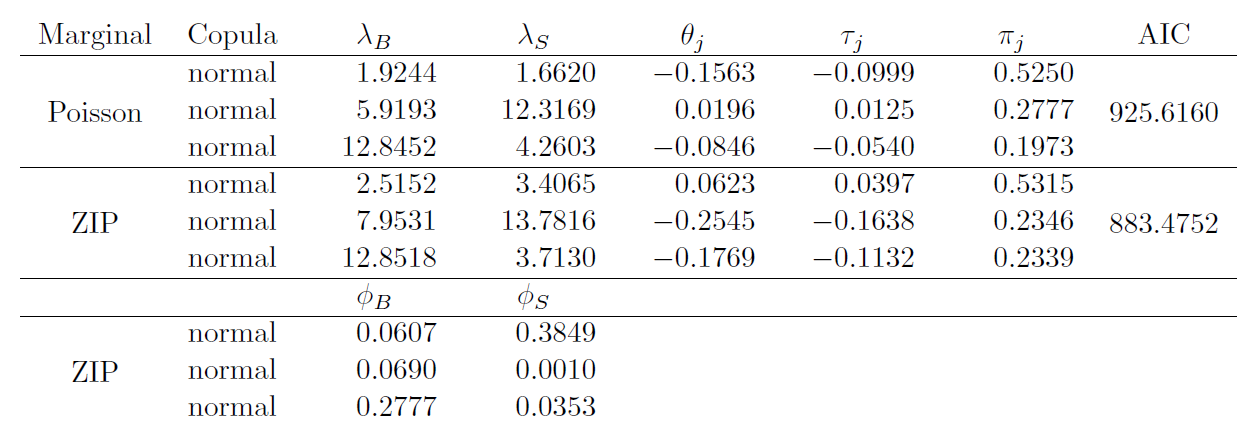
\includegraphics[width=\textwidth]{figures/NTE_080529.png}
        \caption{The fitting result of the stock NTE (2008/05/29)}
    \end{figure}
\end{frame}


\begin{frame}{Stock NTE in 2008/05/29}
    \begin{figure}[!h]
	\begin{subfigure}{.49\textwidth}
		\centering
		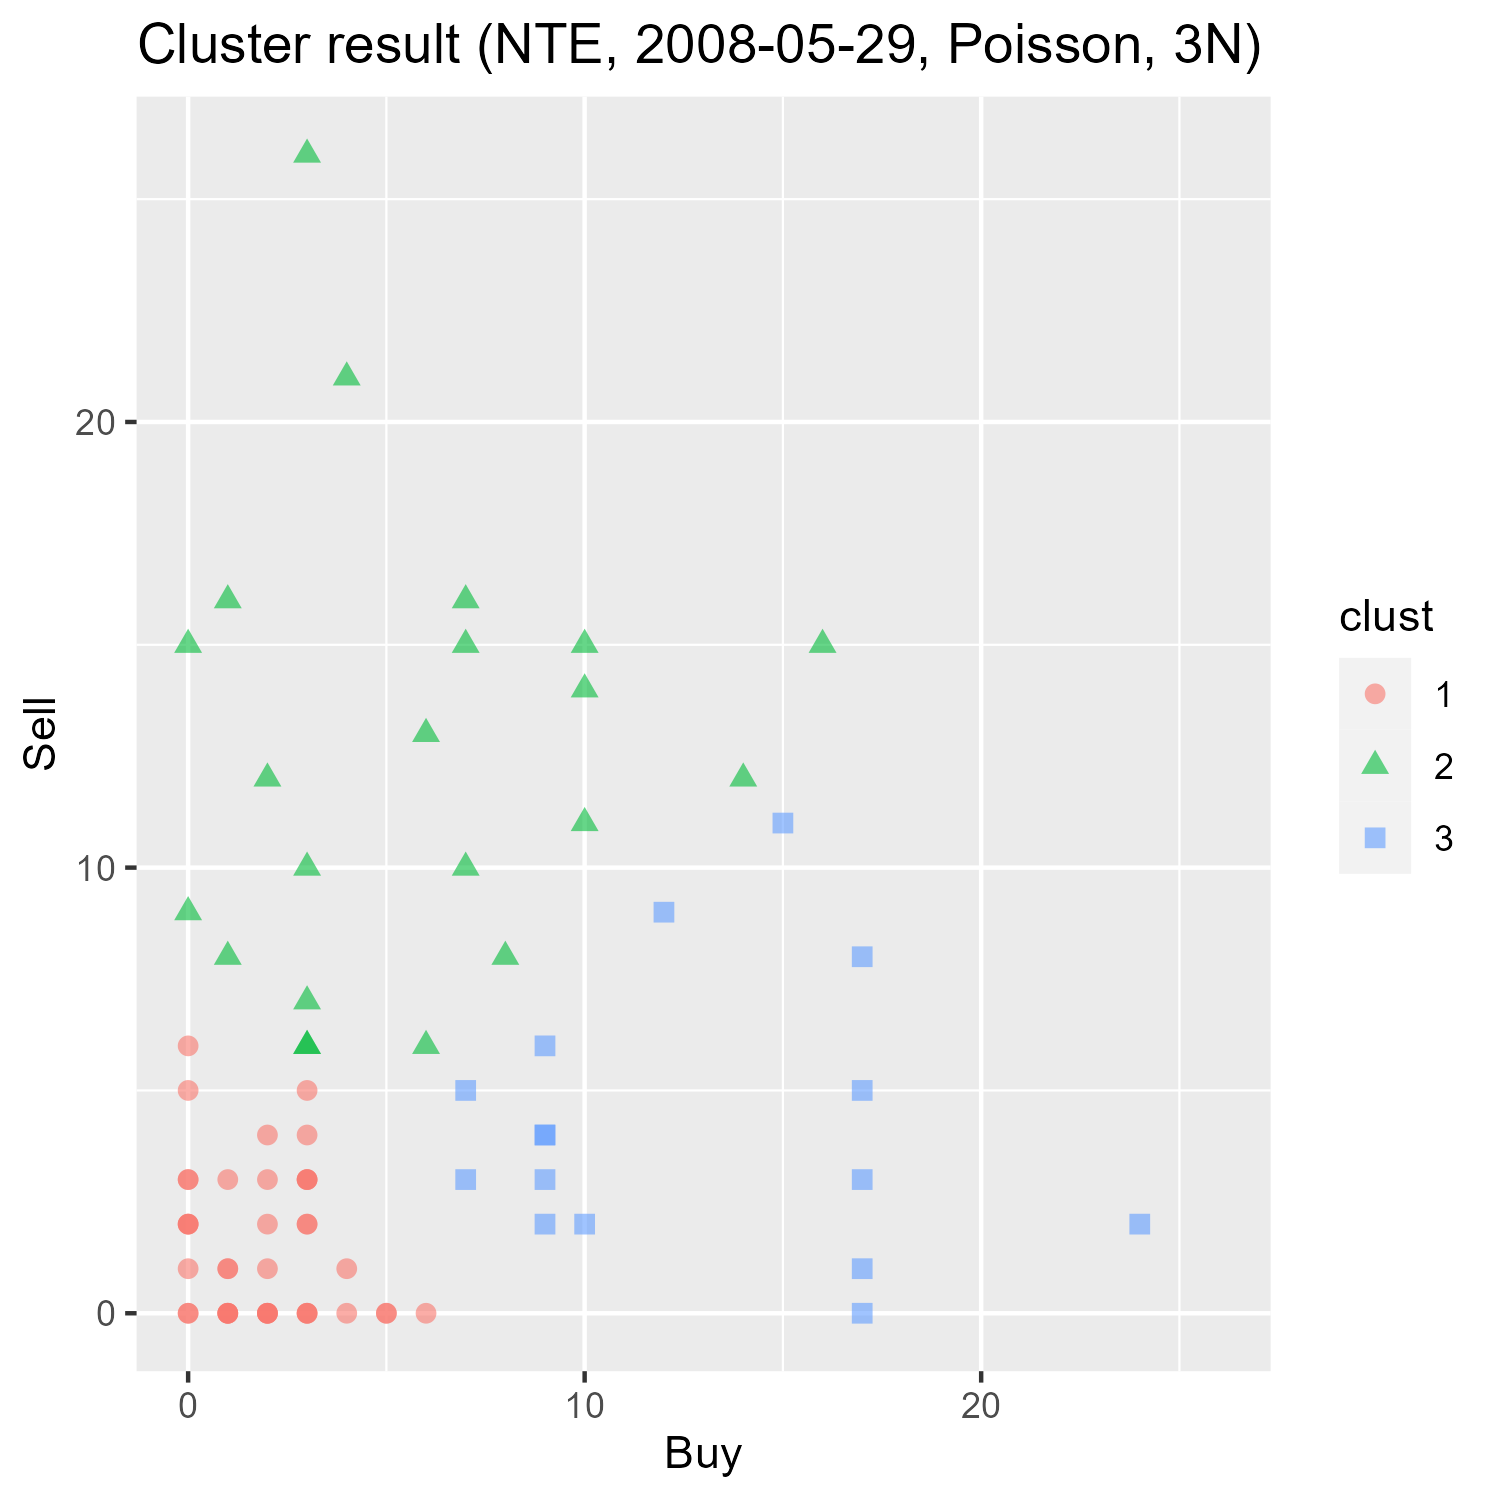
\includegraphics[width=\textwidth]{figures/Scatter_clust(NTE, 2008-05-29, Poisson, 3N).png}
		\caption{Poisson marginal}
	\end{subfigure}
	\begin{subfigure}{.49\textwidth}
		\centering
		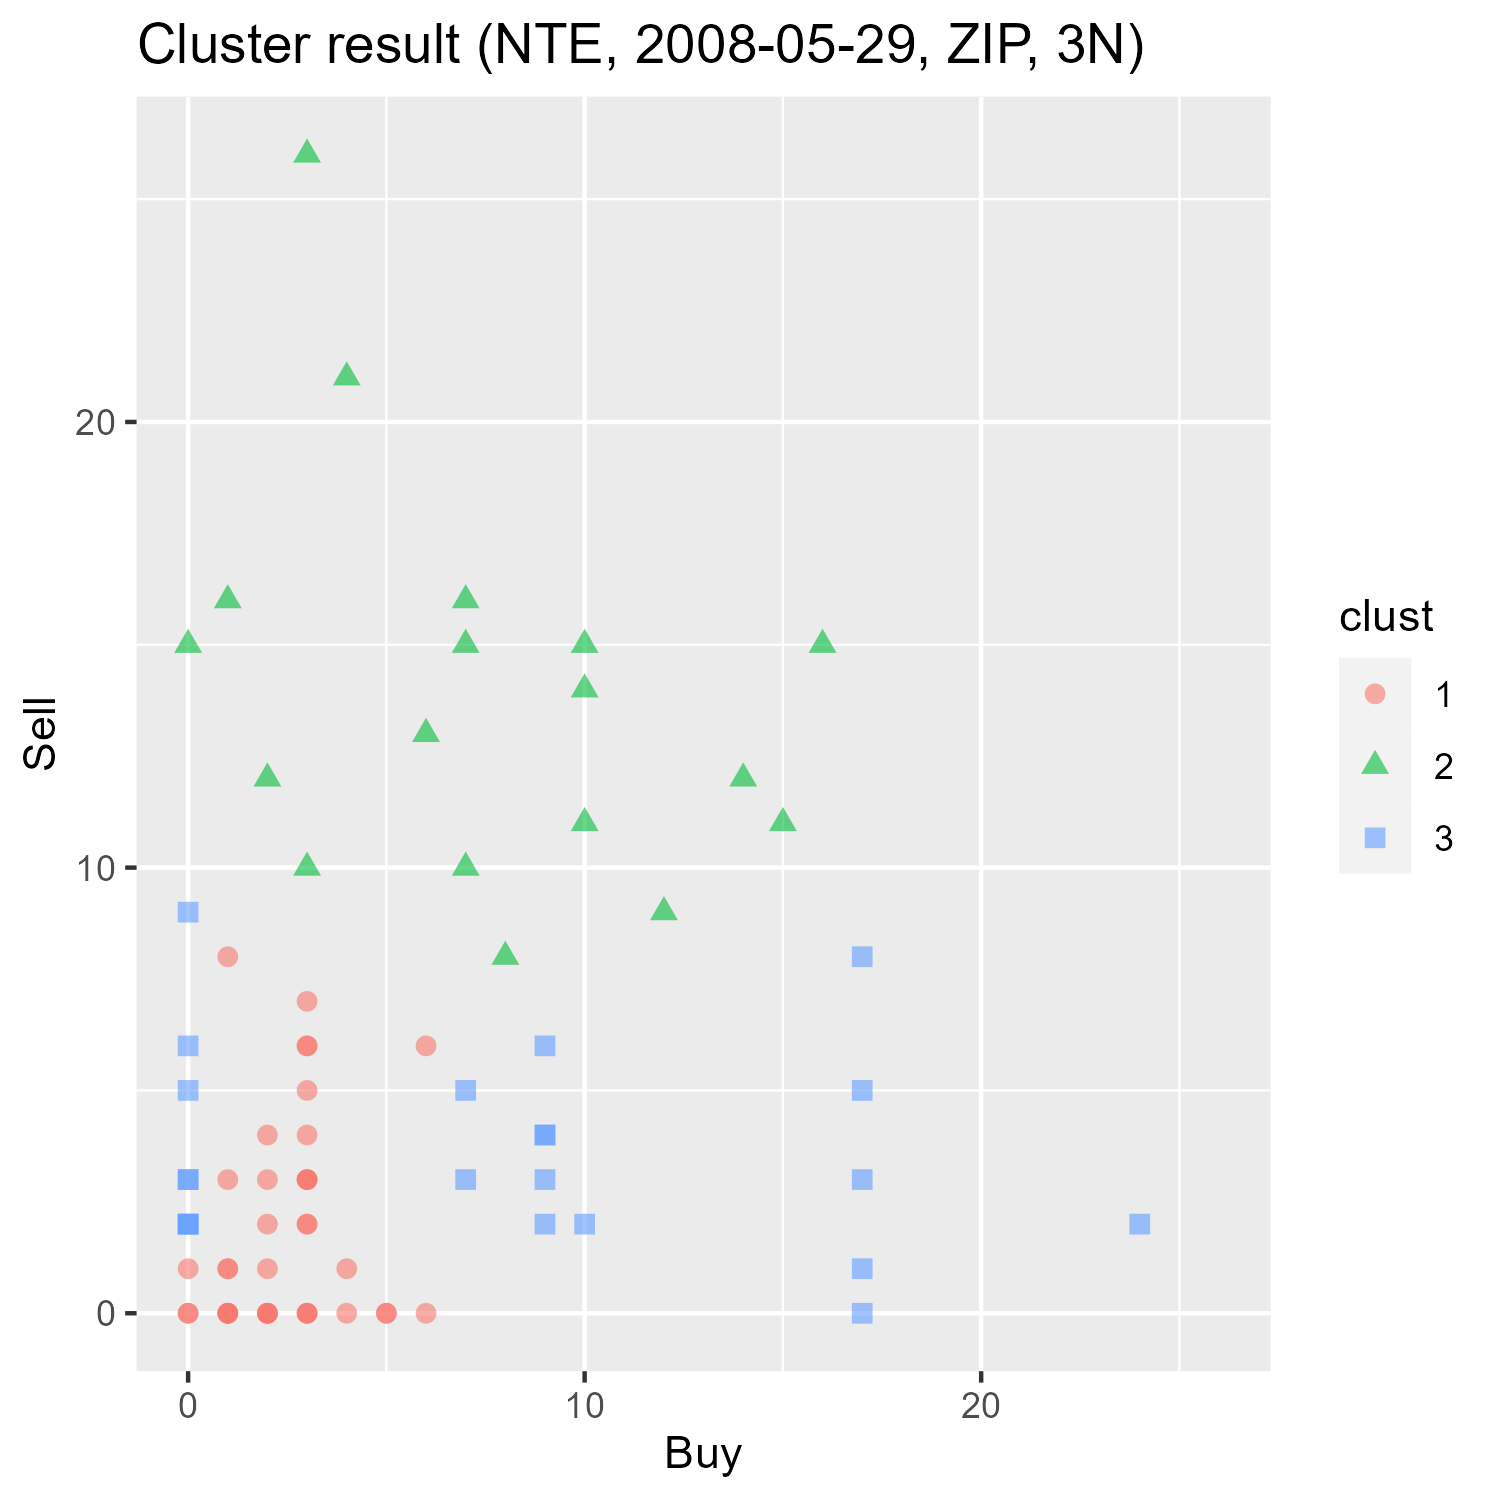
\includegraphics[width=\textwidth]{figures/Scatter_clust(NTE, 2008-05-29, ZIP, 3N).png}
		\caption{Zero-inflated Poisson marginal}
	\end{subfigure}
    \caption{Clustering result of the stock NTE in 2008/05/29 (3 normal)}\label{clust_NTE}
    \end{figure}
\end{frame}


\begin{frame}{Stock NTE in 2008/05/29}
    \begin{figure}[!t]
        \centering
        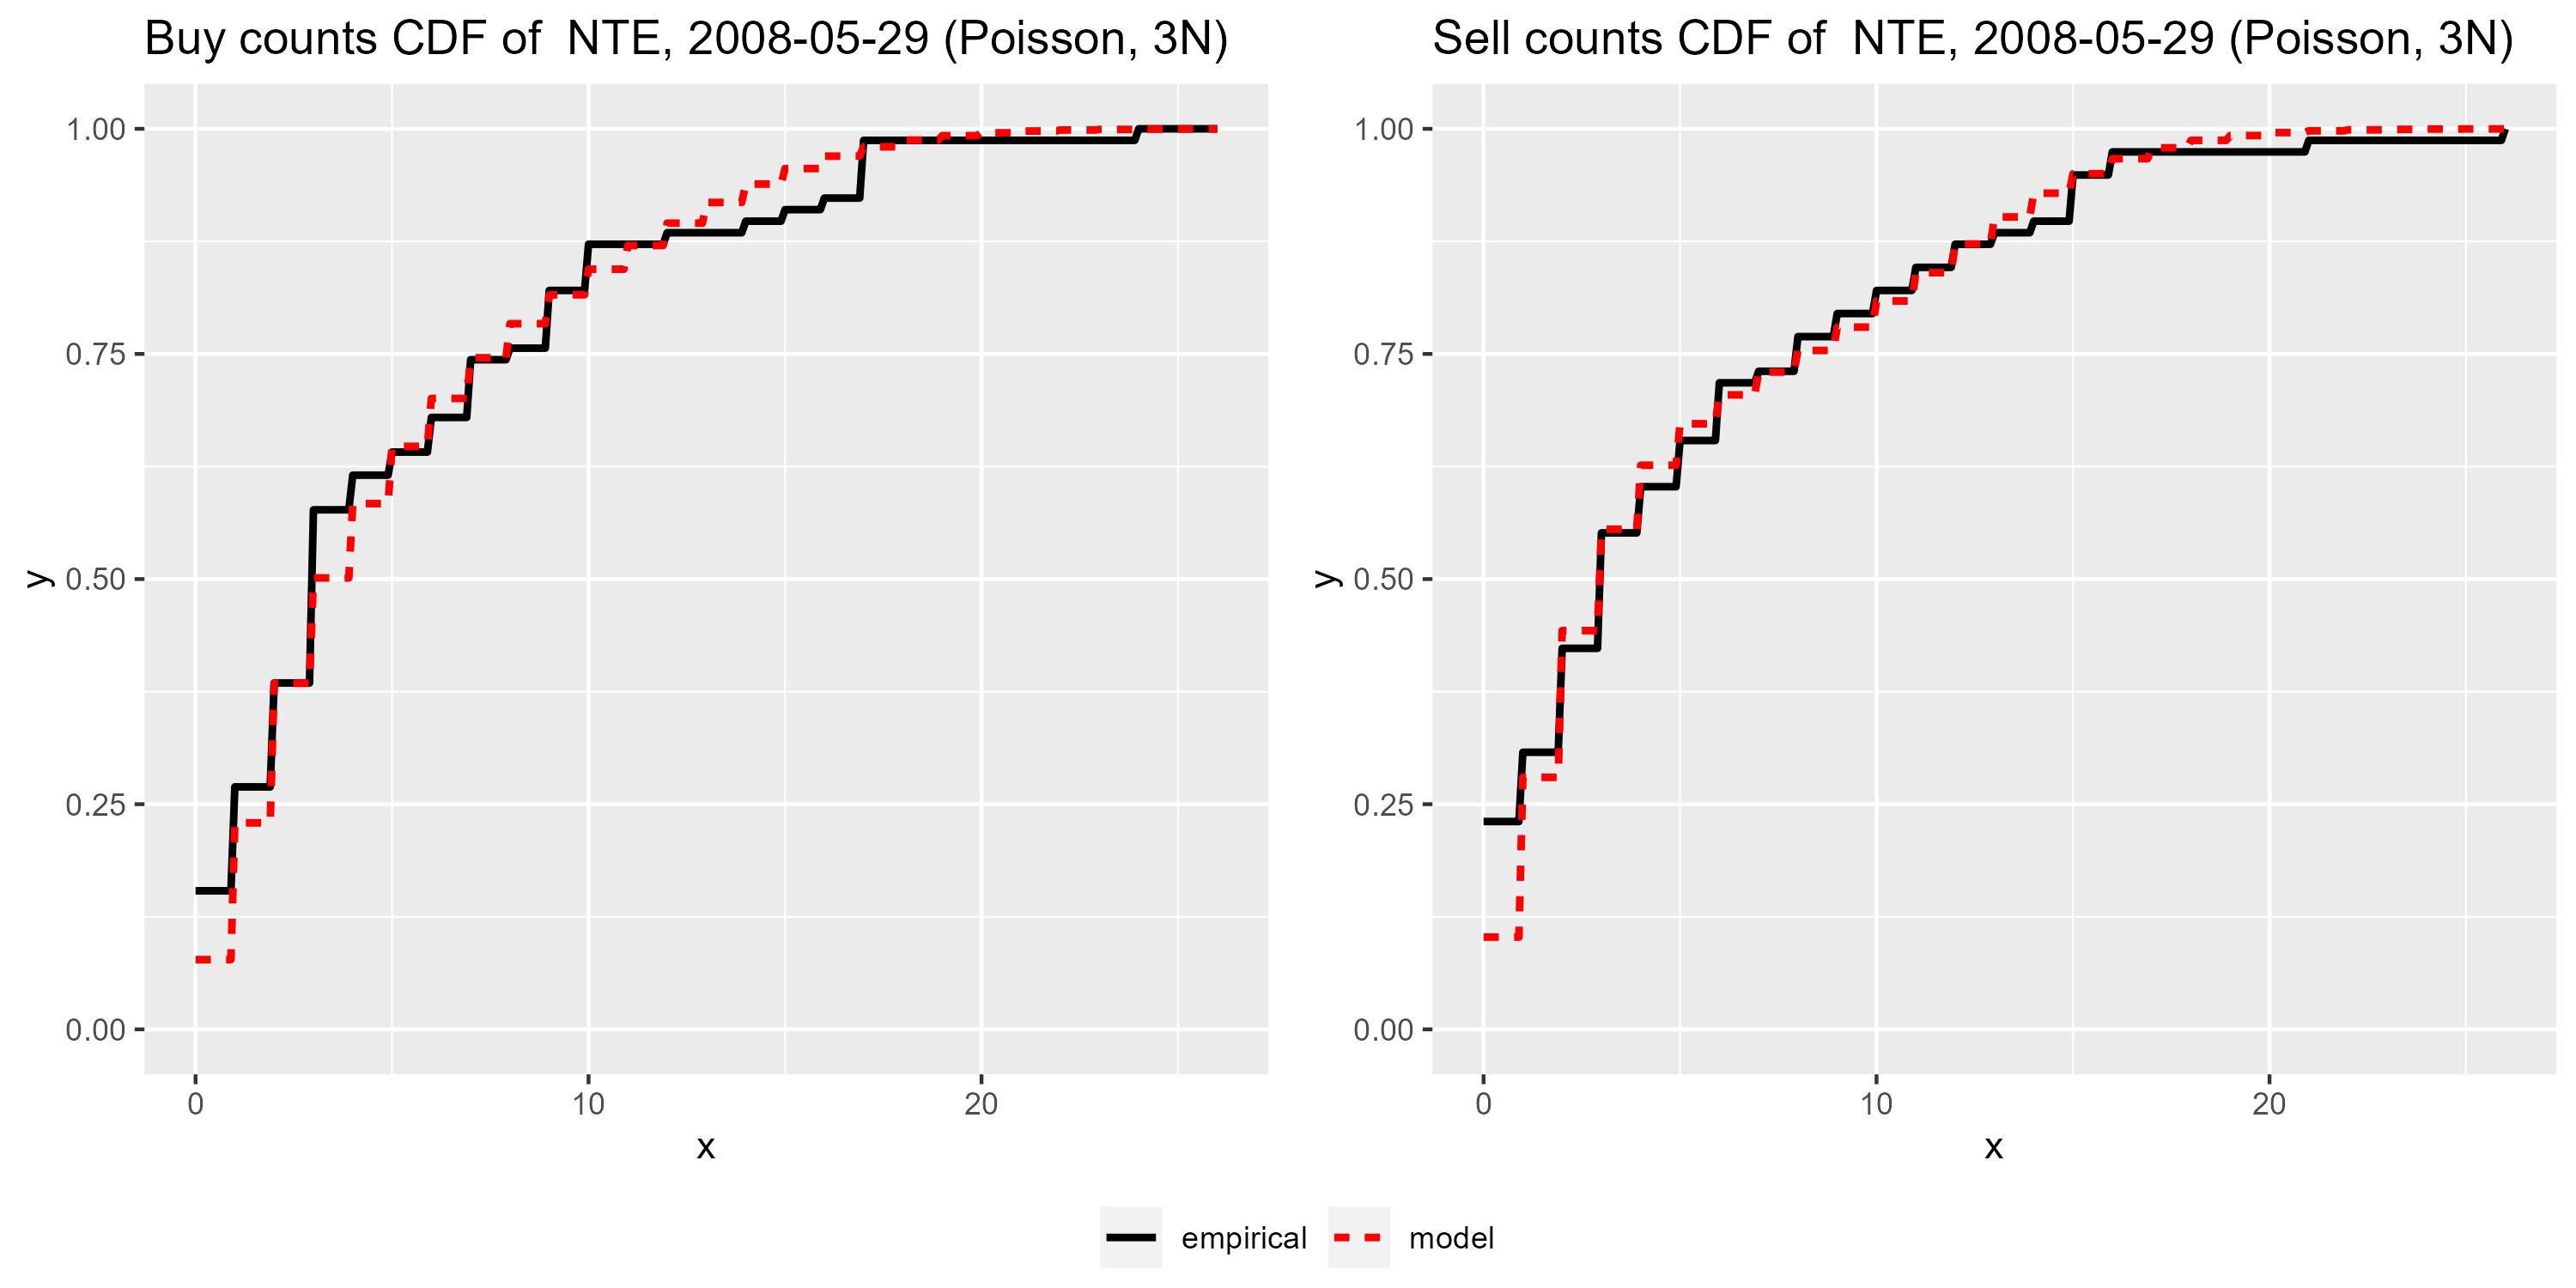
\includegraphics[width=\textwidth]{figures/CDFNTE, 2008-05-29 (Poisson, 3N).png}
        \caption{Marginal cdf of the NTE stock in 2008 (Poisson, 3 normal)}
        \label{poi_NNN_NTE_2008_cdf}
    \end{figure}
\end{frame}

\begin{frame}{Stock NTE in 2008/05/29}
    \begin{figure}[!t]
        \centering
        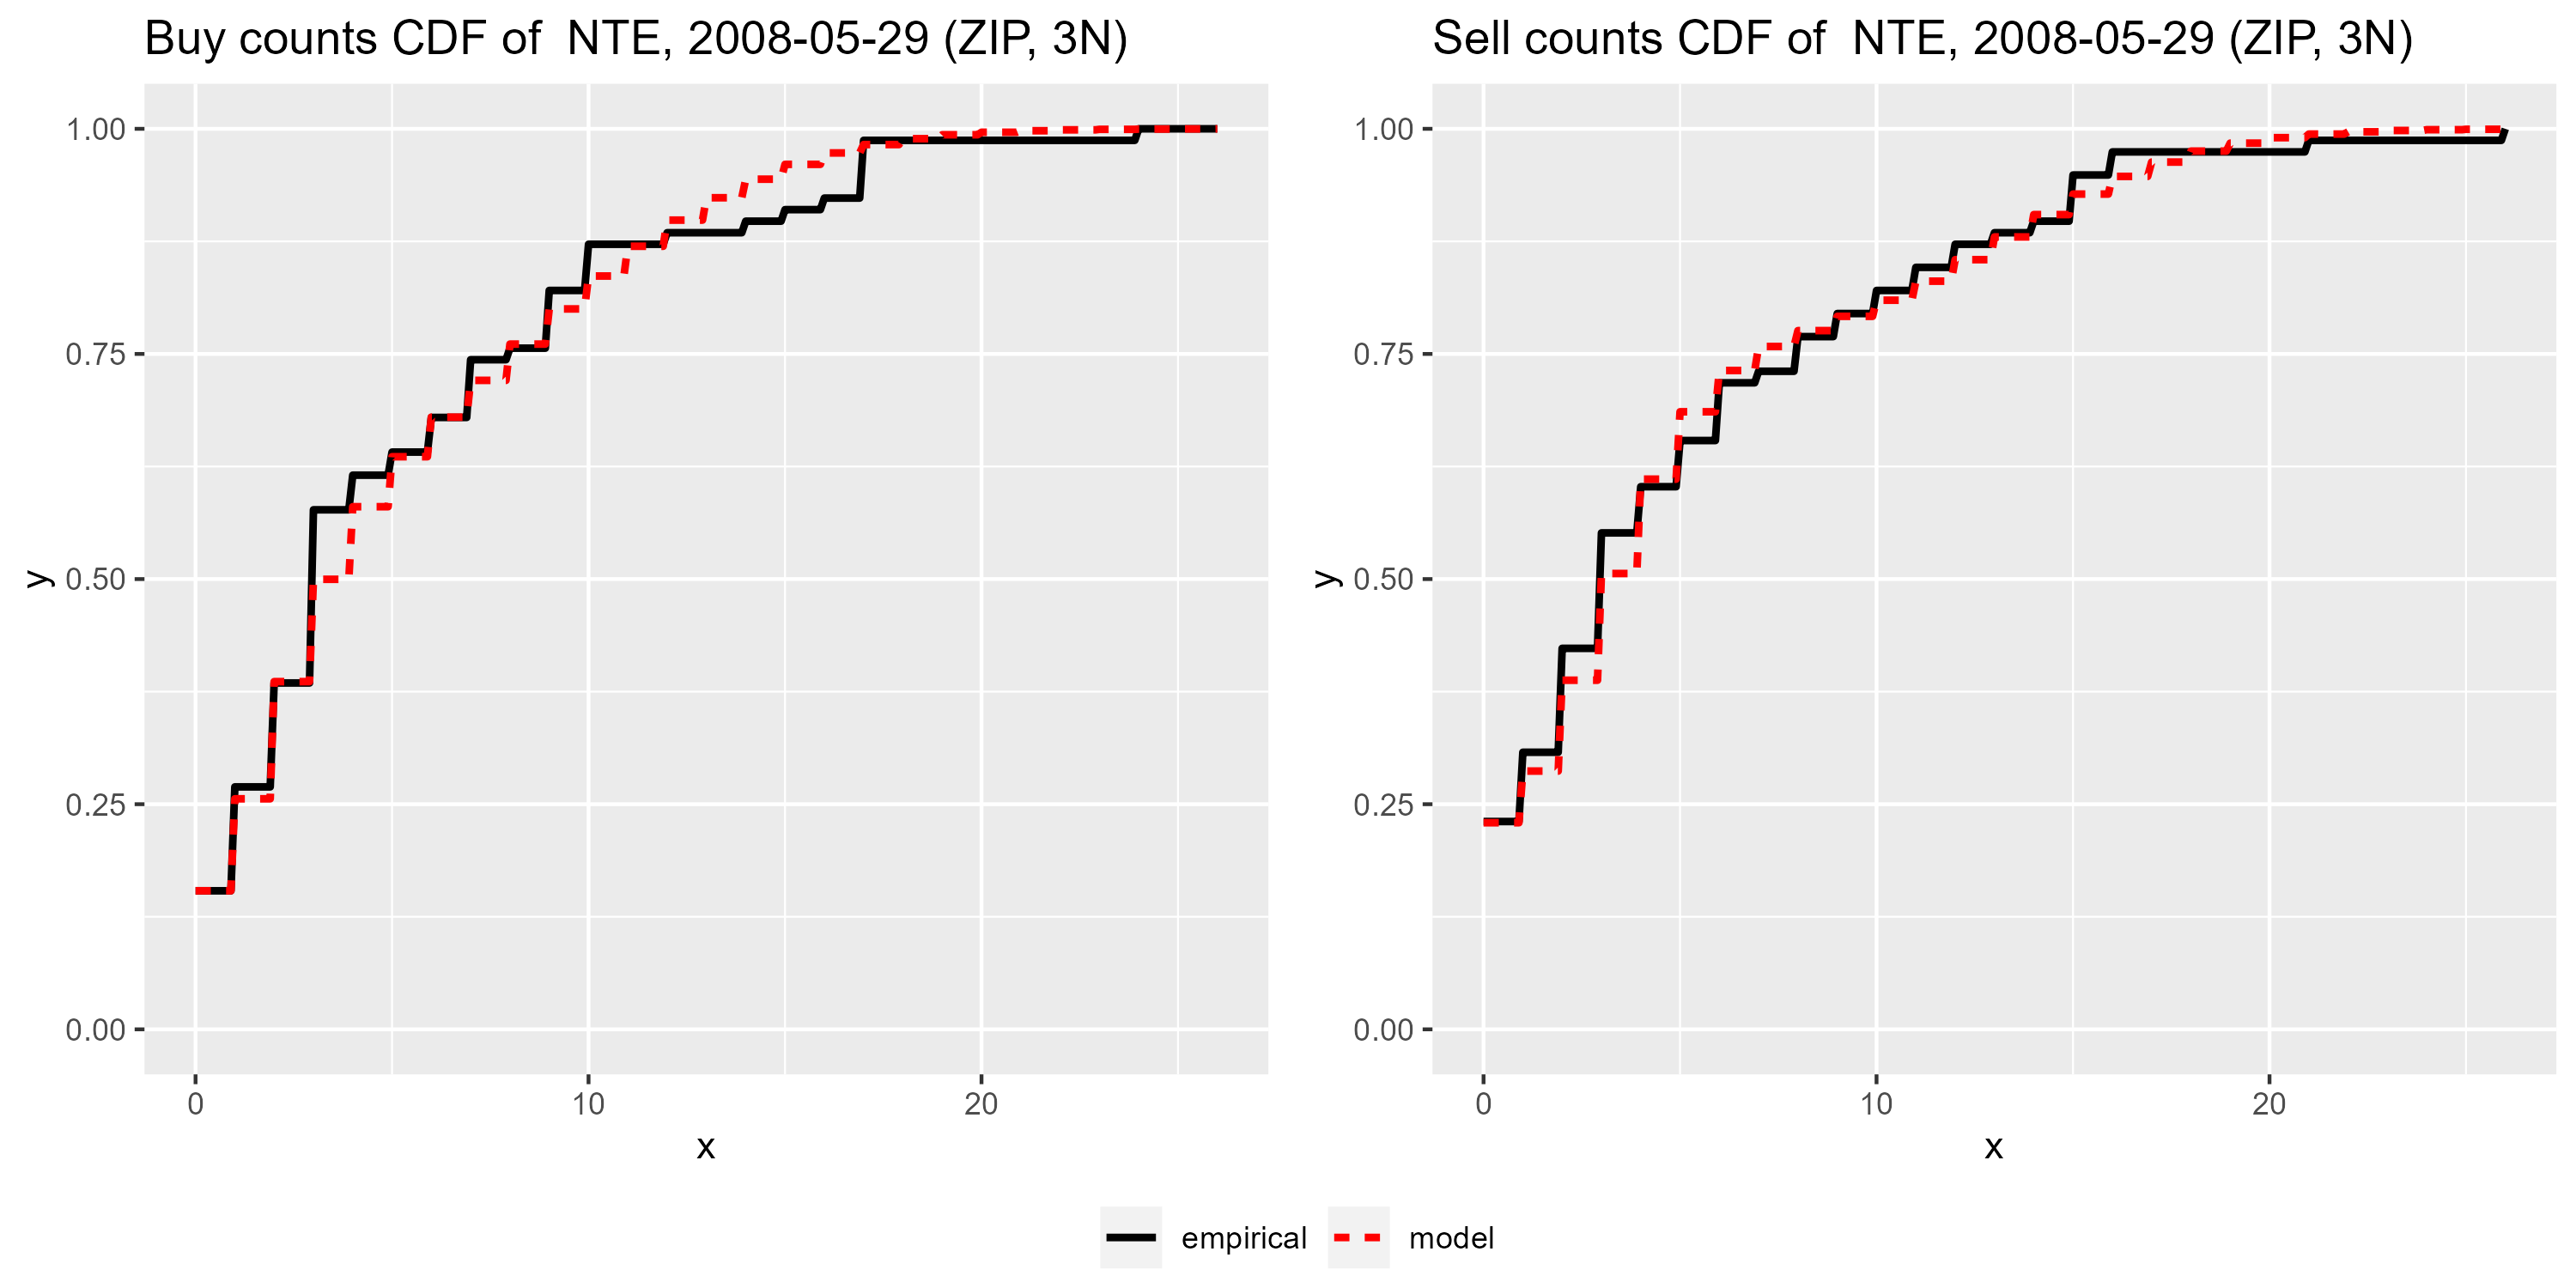
\includegraphics[width=\textwidth]{figures/CDFNTE, 2008-05-29 (ZIP, 3N).png}
        \caption{Marginal cdf of the NTE stock in 2008 (ZIP, 3 normal)}
        \label{zip_NNN_NTE_2008_cdf}
    \end{figure}
\end{frame}

\begin{frame}{Stock NTE in 2008/05/29}
    \begin{figure}[!t]
        \centering
        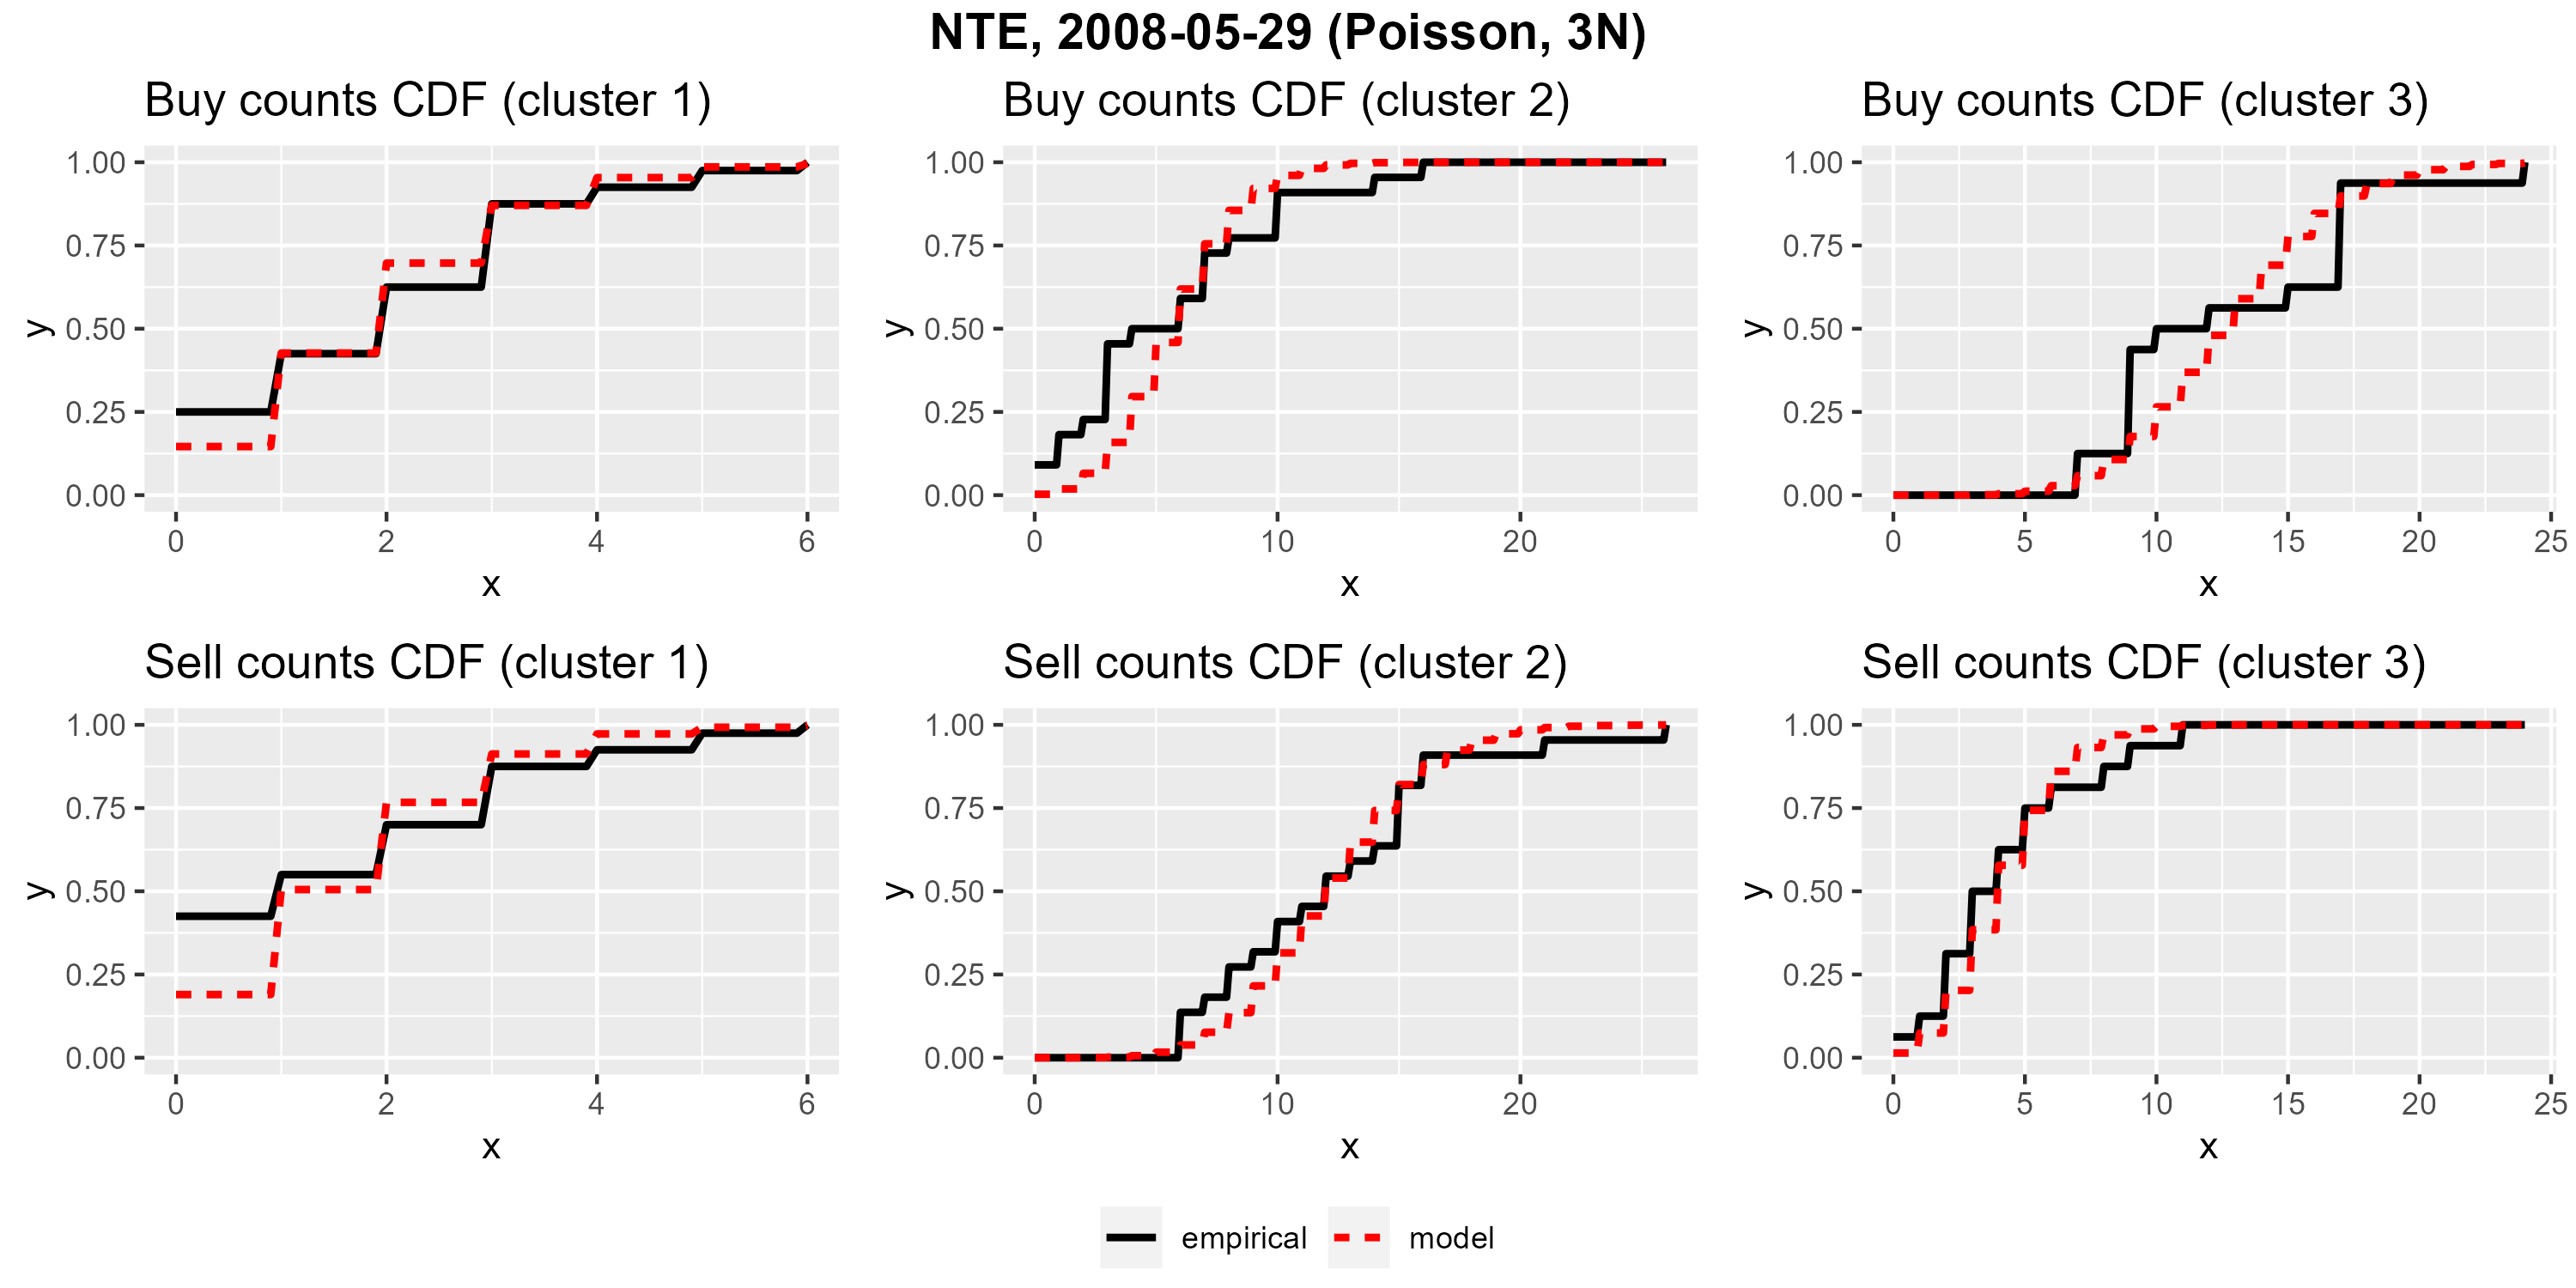
\includegraphics[width=\textwidth]{figures/CDF_sepNTE, 2008-05-29 (Poisson, 3N).png}
        \caption{Marginal cdf of each cluster of the NTE stock in 2008 (Poisson, 3 normal)}
        \label{poi_NNN_NTE_2008_cdf_sep}
    \end{figure}
\end{frame}

\begin{frame}{Stock NTE in 2008/05/29}
    \begin{figure}[!t]
        \centering
        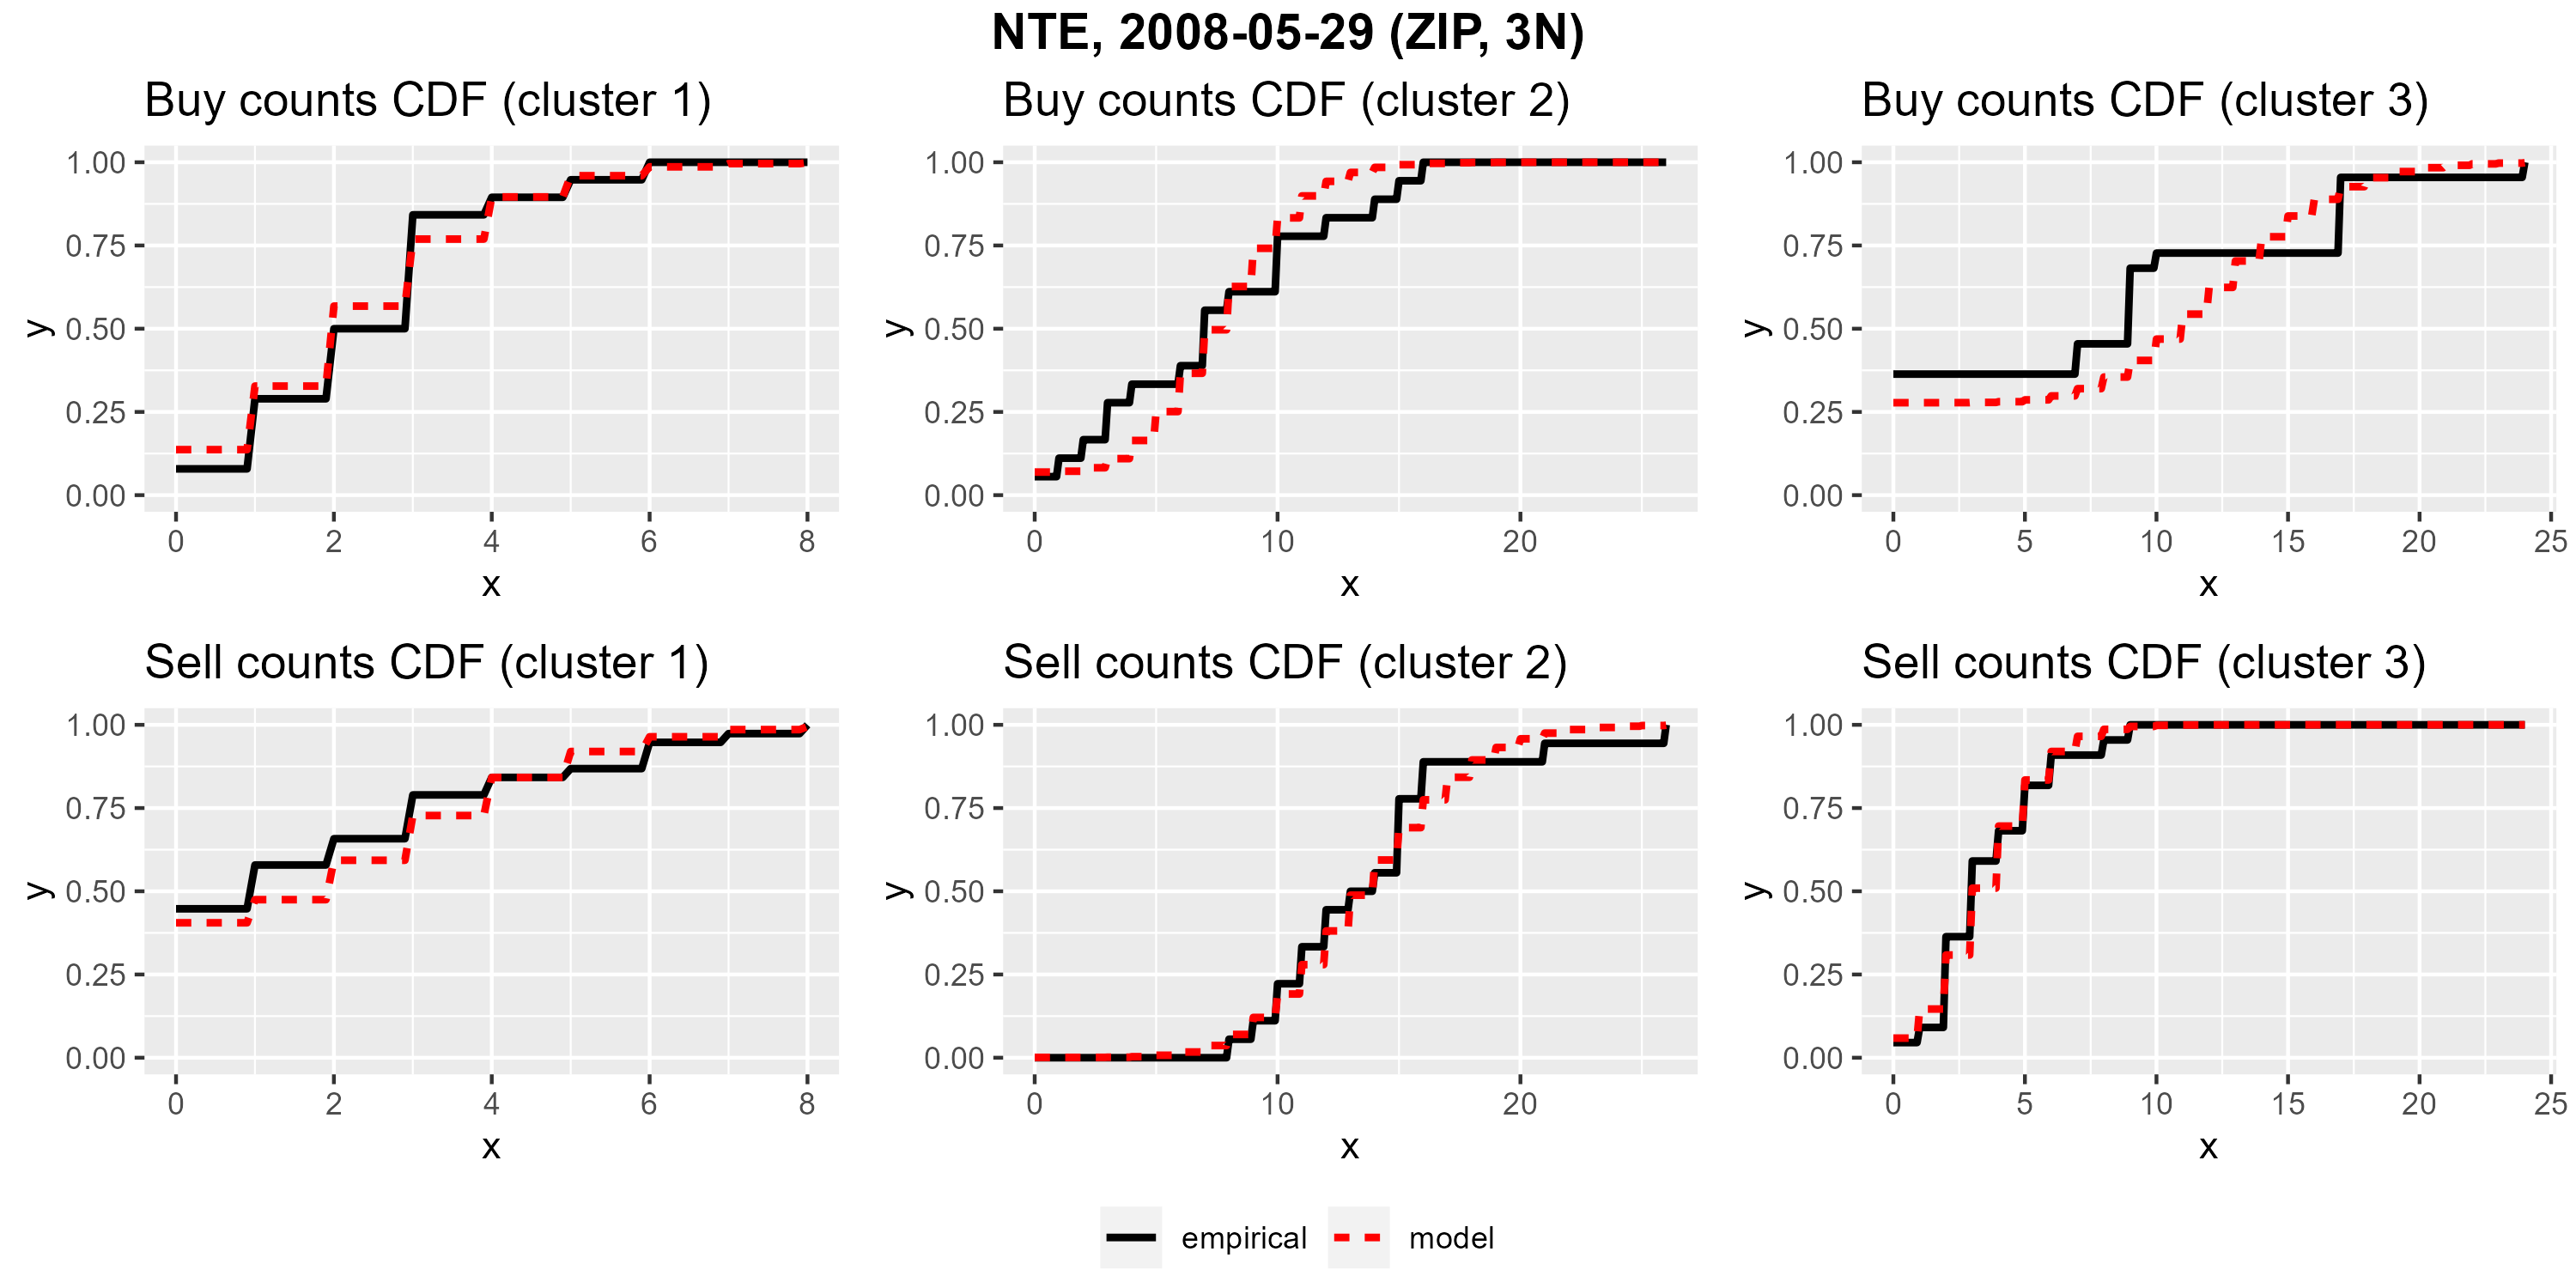
\includegraphics[width=\textwidth]{figures/CDF_sepNTE, 2008-05-29 (ZIP, 3N).png}
        \caption{Marginal cdf of each cluster of the NTE stock in 2008 (ZIP, 3 normal)}
        \label{zip_NNN_NTE_2008_cdf_sep}
    \end{figure}
\end{frame}



\section{Discussion and Future work}

\begin{frame}{Discussion and Future work}
    \begin{itemize}
        \item Proposed a method (co-PIN) to evaluate the PIN model with the correlation structure by using the copula function and the ECM algorithm.
        
        \item We observed a correlation in the PIN model, proving that the independent assumption was too strict.
        
        \item In future work, we aim to modify the code to fit the rotate copula and find a suitable method to obtain initial parameters. 
        
        \item From the empirical studies results, the issue of misspecification in the mixture copula model is also an interesting topic for further research.
    \end{itemize}
\end{frame}

%\section{Reference}

\begin{frame}[allowframebreaks]{Reference}
    \nocite{*}
    \AtNextBibliography{\scriptsize}
    \printbibliography
\end{frame}


% \begin{frame}{Some observation on correlation and counts}
%     \centering
%     \animategraphics[loop,width=\textwidth,controls=all]{1}{figures/freq_corr/freq_cor_}{2002}{2010}
%     %\caption{Relations between correlation and counts}
%     \label{freq_cor_anime}
% \end{frame}

\end{document}
